\documentclass[]{final_report}
\usepackage{graphicx}
\usepackage{hyperref}
\usepackage{siunitx}


%%%%%%%%%%%%%%%%%%%%%%
%%% Input project details
\def\studentname{Oraz Ospanov, Asset Malik, Andrey Yershov}
\def\projecttitle{Data-Driven Control for DC Motors}
\def\supervisorname{Do Duc Ton}

\begin{document}

\maketitle

\pdfbookmark[0]{Table of Contents}{toc}
\tableofcontents
\newpage

%%%%%%%%%%%%%%%%%%%%%%
%%% Your Abstract here

\begin{abstract}

\textbf{\textsl{
This paper describes the work done for the Final Year Project on topic of Data Driven Control for DC motors. Multiple experimental approaches were considered for the project, for instance MATLAB/SIMULINK simulation of the DC motor with different configurations, a setup with an Arduino and DC motor driver, an STM32 micro controller and DC motor driver  and a dSpace DC motor setup. Data on voltage and position relation was collected for all of the mentioned approaches and was analyzed in MATLAB for the Data Driven controller design. The obtained results from comparison of the system identification toolbox generated transfer function with the validation time-position graph was 41.07\% for the STM32 joined with Arduino setup. While better results on transfer-function validation were achieved for the dSpace setup, it was not possible to verify the controller performance for it due to multiple reasons described in the implementation chapter. For the STM32 micro controller setup the robust controller was generated and proved to be fully functional.

}}

\end{abstract}
\newpage

%%%%%%%%%%%%%%%%%%%%%%
%%% Acknowledgments

\chapter*{Acknowledgments}

We would like to thank our project Supervisor Ton Duc Do for support during the project course and providing the lab space and equipment. We thank Mr. Kanat for help with the dSpace setup and comfortable atmosphere in the lab.

%%%%%%%%%%%%%%%%%%%%%%
%%% Introduction

\chapter{Introduction}
\section{Model Based Control}

The modern control theory, also known as Model Based Control has been used both for linear and non-linear systems extensively since 1960. The Model Based Control is, as could be guessed from it's name, relies solely on the model of the plant for further controller design. However, there is usually no chance of creating an exact plant model for the system, as well as no efficient way of creation high accuracy plant model using the classical model based control \cite{hou2013model}. Moreover, the possible plant model errors have to be considered when designing the controller from the plant model, what requires additional resources and time to provide robustness of the controller. All of the used control design methods heavily rely on the assumptions of an accurate plant model design. This means that in case if unmodeled dynamics occurs, the controller is believed to be unable to provide further handling of the dynamics. As could be seen in Fig. \ref{fig:mbcsctruct}, the Model Based Controller design starts from the assumptions about the model plant and is directed at regulation of the plant \cite{hou2013model}.

\begin{figure} [h!]
\centerline{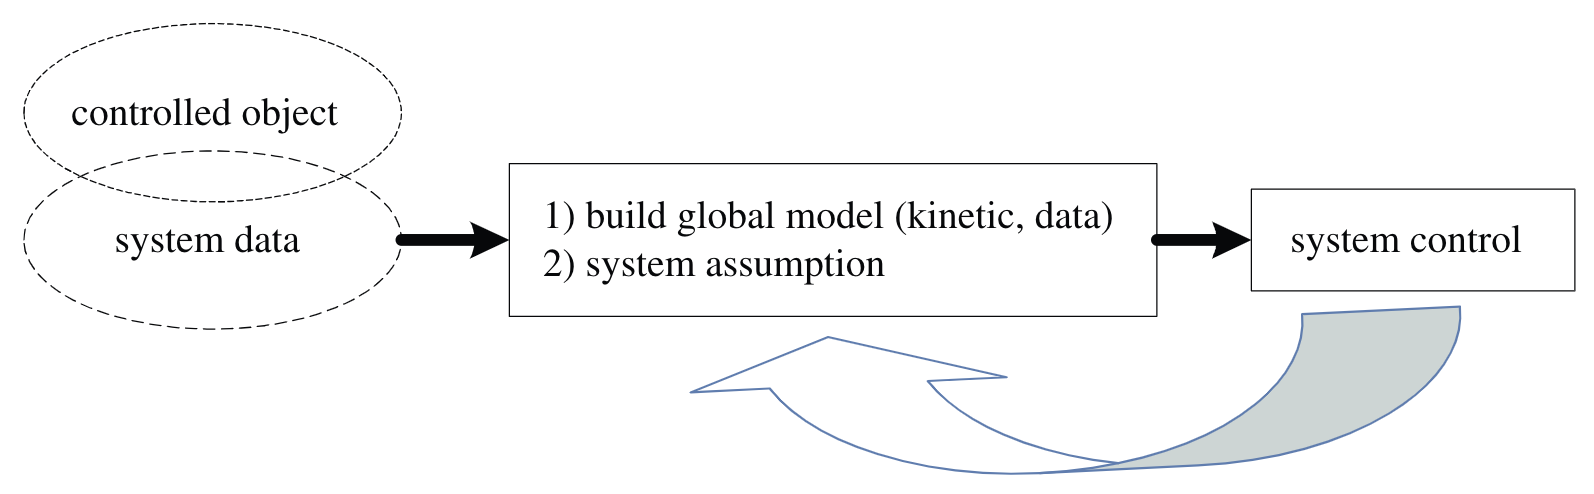
\includegraphics[width=.65\textwidth]{Screenshots for paper/1.png}}
\caption{Common structure of the Model Based Control \cite{hou2013model}}
\label{fig:mbcsctruct}
\end{figure}

\section{Data Driven Control}

Opposed to the Model Based Control, Data Driven control is becoming more popular. \cite{hou2013model} suggest the following definition for Data-Driven control: "Data-driven control includes all control theories and methods in which the controller is designed by directly using on-line or off-line I/O data of the controlled system or knowledge from the data processing but not any explicit information from mathematical model of the controlled process, and whose stability, convergence, and robustness can be guaranteed by rigorous mathematical analysis under certain reasonable assumptions". Data-Driven control for various purposes is becoming the superior method in systems where the model is not available or is changing over the course of life cycle, i.e. adaptability is necessary. This implies that motors and other motile systems are the ones which need Data-Driven control the most. Data-Driven controller design method allows to bypass the tedious system identification step. However, as every machine learning problem, it requires big amounts of data. This becomes less of a problem year by year, as every industry, be it information technology or metallurgy, is becoming more and more digitized and thus produces vast amounts of data. This data has a vast potential of improving the current processes if processed correctly. The data gathered from the system behaviour is used to identify the controller. In this paper, we investigate the application of data-driven control to the control of DC motor drives and experiment with data-driven controller estimation using reinforcement learning. As it could be seen on the figure \ref{fig:ddcwork}, \cite{naung2018a} outlined the Data-Driven Control workflow in a cycle figure.

\begin{figure} [h!]
\centerline{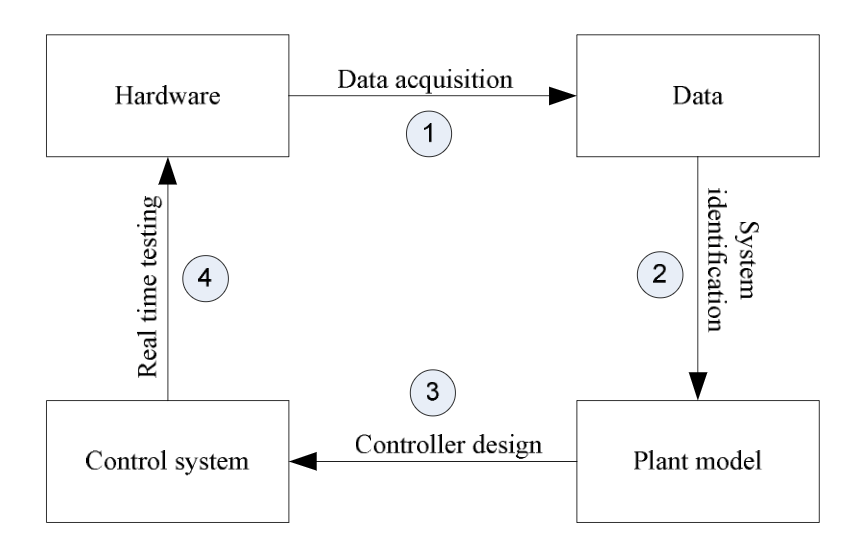
\includegraphics[width=.5\textwidth]{Screenshots for related work/ddc process.png}}
\caption{Data-Driven Control setup workflow \cite{naung2018a}}
\label{fig:ddcwork}
\end{figure}

\section{Motivation for Data-Driven control for DC motors}
DC motors are an inseparable part of modern motile systems in engineering and robotic system control. They are efficient and are able to be controlled in various ways. However, there may be different circumstances when the DC motor system is exposed to abrupt load changes, electromagnetic disturbances and highly varying inputs \cite{naung2018a}. These circumstances are unlikely to be considered during the factory manufacturing step of the motors, and the Data-Driven controller design could help with understanding the motor behaviour at those circumstances and dealing with them. Further, the Data-Driven controller design for DC motors could be used as a calibration process for DC motors in robotic systems, which has served for a prolonged period of time and experience wear-out issues. For safety considerations, better performance and controllability a robust controller must be designed and maintained for a given DC motor. As was discussed earlier, the recent deep learning achievements provide us with an ability to do so without having the knowledge about the architecture of the DC motor. The controller is designed relying on the data from input voltage and output position. 

In this paper, multiple approaches to data-driven control are going to be tested with DC motors. First, the DC motor is going to be simulated using MATLAB/SIMULINK  platform in three scenarios: Open Loop DC motor with Pulse Width Modulation (PWM) input, Closed Loop DC motor with known parameters and Closed Loop DC motor with unknown parameters. The difficulty of the controller design thus will increase in 3 steps as well. Next, the plan is to setup the physical model using a simple DC motor with unknown parameters with an encoder (to control its position) and an Arduino Uno connected to the PC as a micro controller for the DC motor driver. With the MATLAB model the data is to be collected with a number of signals generated by Signal Builder tool (step, sine, triangular, nonlinear etc.). The collected data is then to be processed to build a controller for that DC motor. To demonstrate that this approach is applicable to any DC motor system, even the larger and more complicated ones, the physical model is to be tested on the dSpace DC motor.After the data collection process is finished, the data is to be used to design the controller. The initial aim of this project is to compare the available approaches, namely the ones provided by MATLAB: System Identification Toolbox and NARX Neural Network. After this is complete, a plug-and-play reinforcement learning setup is to be designed to generate controller for any given DC motor.

\chapter{\label{chapter2} Related Work}

\section{Algorithms for Data-Driven control}
The article written by Naung et al. \cite{naung2018a} is closely related to our work by the research aims and methods. Authors present Data-Driven Control used for system parameters identification, an approach that we are planning to use. The main goal of the paper is to perform system identification utilizing the data driven system control of the DC motor, with ultimate generation of the transfer function suitable for robust control of the plant. For this purpose, authors use MATLAB to create the Simulink model of the DC motor (Figure \ref{fig:dcsimulink}) and calculate the proportional-integral-differential (PID) controller according to the obtained models.

\begin{figure} [h!]
\centerline{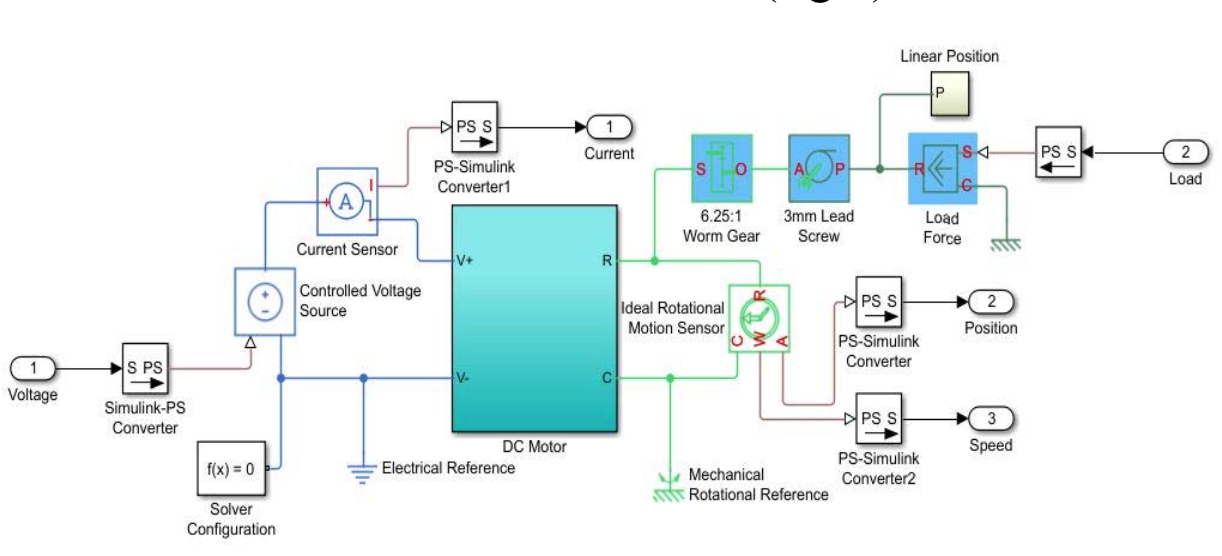
\includegraphics[width=.75\textwidth]{Screenshots for related work/1.png}}
\caption{Simulink diagram of simscape physical plant DC motor \cite{naung2018a}.}
\label{fig:dcsimulink}
\end{figure}

Authors compare the performance of the nonlinear autoregressive exogenous inputs (NARX) artificial neural network and nonlinear black-box model structures, summarized in Figure \ref{fig:pidcomparison}. They conclude that the proposed control method performs with acceptable accuracy and is utilizable with more complex dynamic systems.

\begin{figure}
\centerline{
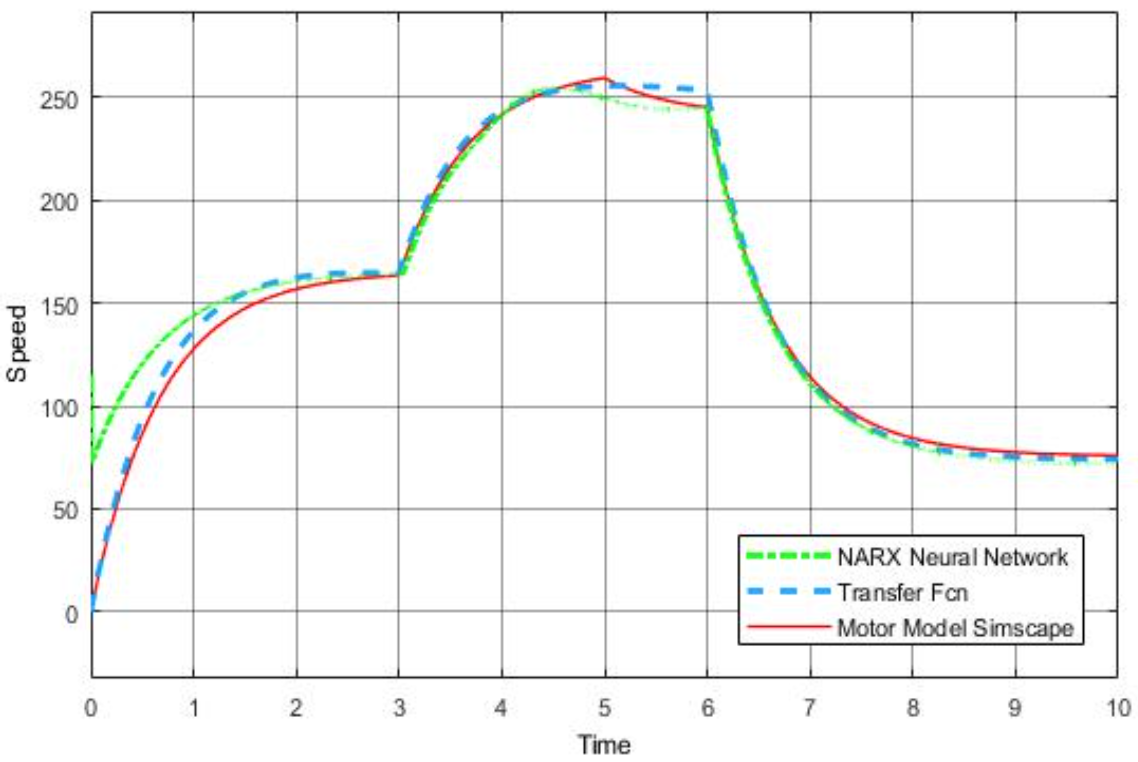
\includegraphics[width=.47\textwidth]{Screenshots for related work/2.png}\hfill
\label{NARX ANN}
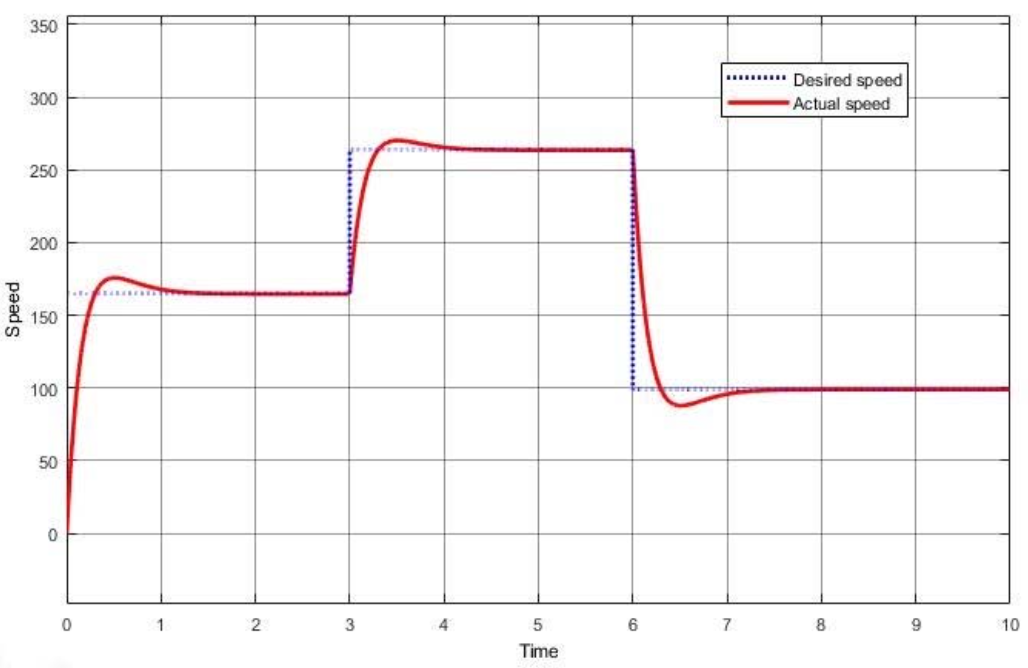
\includegraphics[width=.49\textwidth]{Screenshots for related work/3.png}
\label{PID controller}
}
\caption{Results of the speed response of the DC motor using NARX Neural Network and PID controller \cite{naung2018a}.}
\label{fig:pidcomparison}
\end{figure}

Coulson, Lygeros, and Dorfler introduce novel data-enabled predictive
control (DeePC) algorithm \cite{coulson2019data}, that utilizes real-time feedback of the system, and is able to drive the system along a desired trajectory with given system constraints. The DeePC  algorithm  was  applied  to unknown linear time-invariant (LTI)  system  and was compared to classical Model  Predictive  Control (MPC) algorithm. Authors state that the DeePC was created with thinking from a behavioural systems theory perspective. The algorithm description is provided in both mathematical proof form and a pseudo-code description of the algorithm steps. As an example of sophisticated nonlinear application of the DeePC, a case, a regularized version of the algorithm was simulated on  stochastic nonlinear quadcopter dynamics, illustrating its capabilities beyond deterministic LTI systems - figure \ref{fig:quadsim}.

\begin{figure} [h!]
\centerline{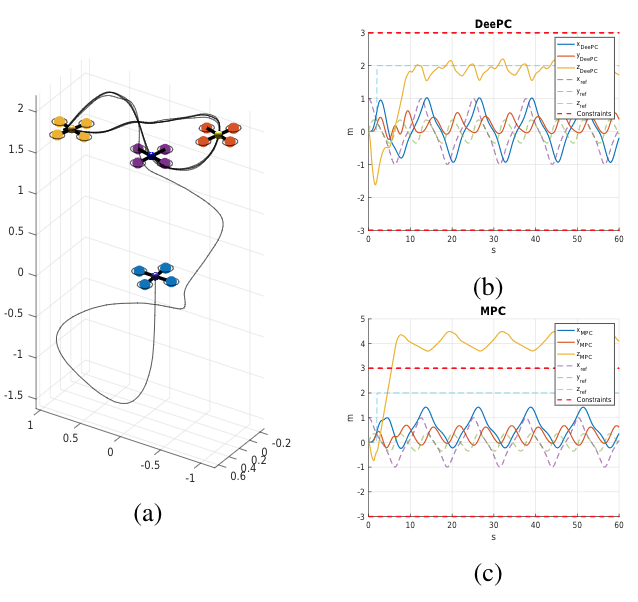
\includegraphics[width=.75\textwidth]{Screenshots for related work/5.png}}
\caption{Figure (a): three dimensional plot of the trajectory of the quadcopter at different instances of time controlled with DeePC.  Figure  (b)  and  (c):  trajectories  of  the  spatial  coordinates  when  controlled  by  DeePC  and  MPC,  respectively. The horizontal red dashed lines represent constraints.
\cite{coulson2019data}}
\label{fig:quadsim}
\end{figure}

A recent work by Carlet et al. \cite{carlet2020data} utilizes the aforementioned DeePC algorithm in a setup with motors. This is an important article for our project, as it explores predictive current control for permanent  magnet synchronous motor drives - a topic closely related to ours. Authors utilize two  of  the  most  popular data-driven   algorithms - the   Subspace Predictive  Control  algorithm  and  the  Data-Enabled  Predictive Control  algorithm. Current  controller  design  procedure for both methods is discussed and presented in detail. Simulation results are reported to be comparably robust and with strong correlation for both of the unconstrained  and  constrained  versions  of  the  data  driven  methods, as it could be seen in figure \ref{fig:controllercomp}.

\begin{figure} [h!]
\centerline{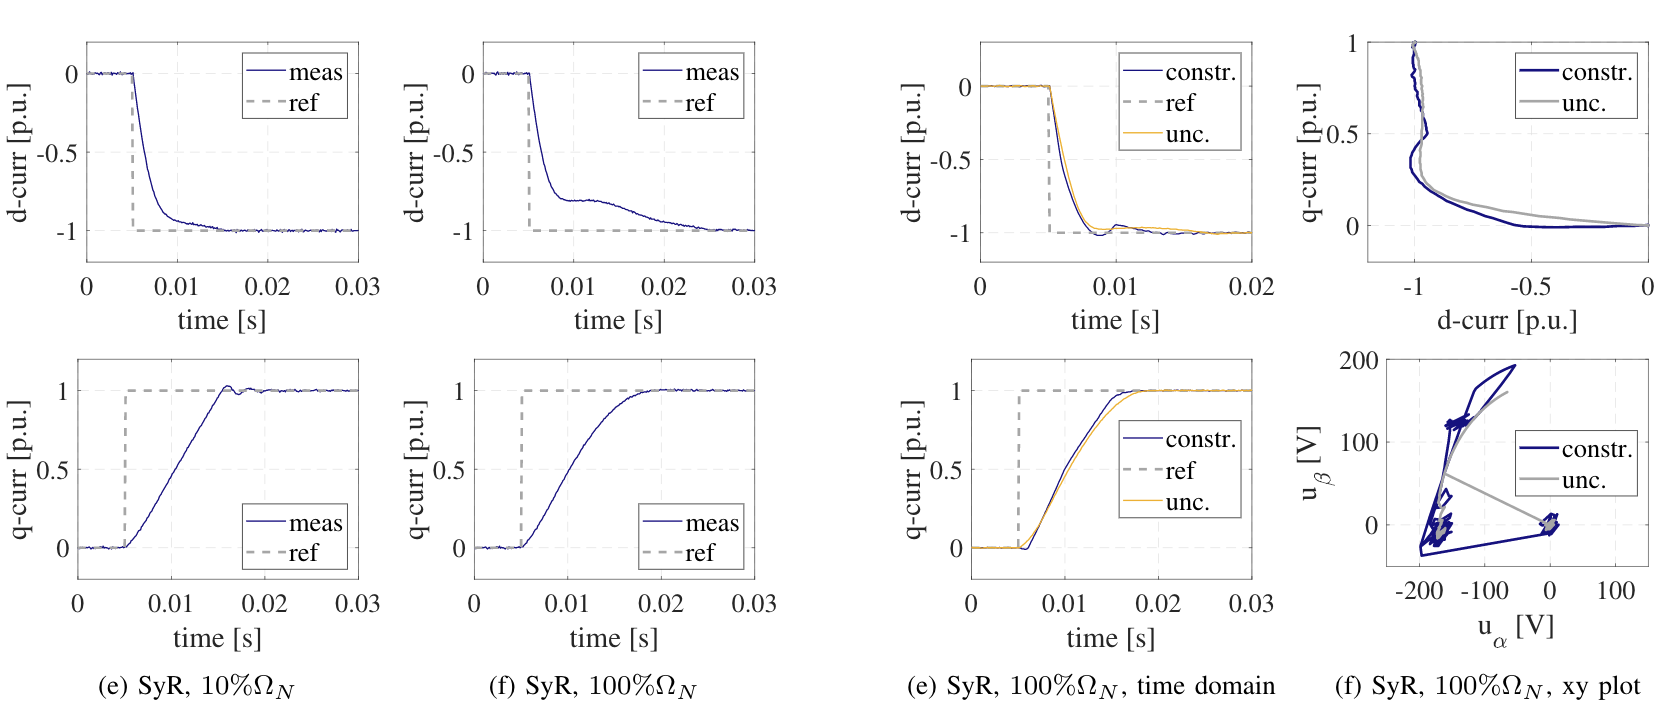
\includegraphics[width=.95\textwidth]{Screenshots for related work/4.png}}
\caption{Step response of SPC data-driven current controllers
\cite{carlet2020data}}
\label{fig:controllercomp}
\end{figure}

Hou and Wang created a canonical survey paper in the field in 2013 \cite{hou2013model}. Almost every other related work cites this paper, as it contains fundamental definitions for the Data driven control and its applications. The paper begins with a brief description and comparison of Model based control theory and Data driven control theory. Motivation for the data based control is stated as well. Further, they state the focus of data-driven control theory in terms of objects that could be controlled with the use of it. For the rest of the survey paper authors explore the recent advances in DDC and discuss the perspectives of future related work. They conclude with categorization of different available Data-driven techniques according to required usage. However, the survey's drawback is that most of the methods are currently outdated, as this is a fast evolving field. The general introductory information provided by the authors is nevertheless valuable.



Next article by Hanke, Wallscheid and Bocker \cite{hanke2019continuous}  introduces Permanent Magnet Synchronous Motor ripple avoidance using DDC. It also compares three types of linear controllers and the input/output data.

\begin{figure} [h!]
\centerline{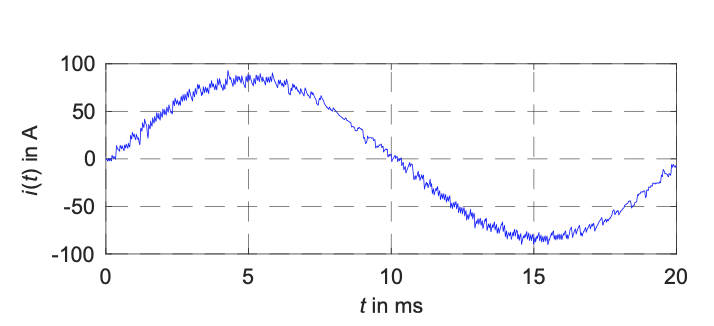
\includegraphics[width=.75\textwidth]{Screenshots for related work/Asset p1/Asset p1p1.png}}
\caption{CCS-MPC at 60A
\cite{hanke2019continuous}}
\label{fig:p1p1}
\end{figure}

\begin{figure} [h!]
\centerline{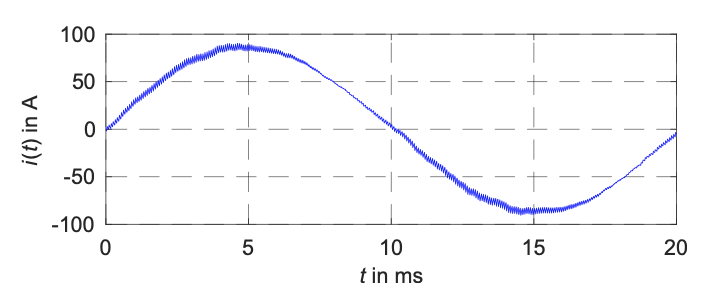
\includegraphics[width=.75\textwidth]{Screenshots for related work/Asset p1/Asset p1p2.png}}
\caption{FOC at 60A
\cite{hanke2019continuous}}
\label{fig:p1p2}
\end{figure}

\begin{figure} [h!]
\centerline{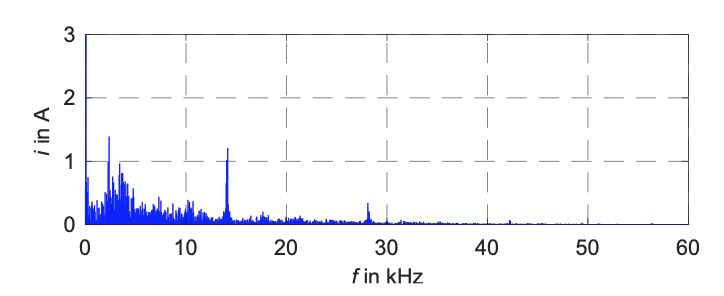
\includegraphics[width=.75\textwidth]{Screenshots for related work/Asset p1/Asset p1p3.png}}
\caption{CCS-MPC at 60A
\cite{hanke2019continuous}}
\label{fig:p1p3}
\end{figure}

\begin{figure} [h!]
\centerline{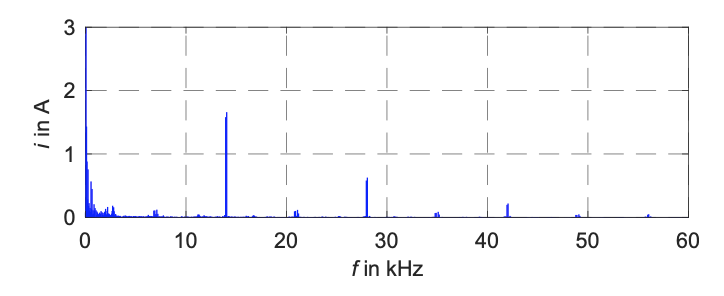
\includegraphics[width=.75\textwidth]{Screenshots for related work/Asset p1/Asset p1p4.png}}
\caption{FOC at 60A
\cite{hanke2019continuous}}
\label{fig:p1p4}
\end{figure}

We can clearly see that total harmonic distortion of the FOC system is smaller and that CCS-MPC only better at those special harmonics of the three phase system.

Article \cite{de2019a} discusses the important attributes for systems with data-driven control: Stabilization, Optimality, and Robustness. Authors argue that it is possible to create a linear approximation of a non linear closed loop system using only data-dependant linear matrix equations. 

Article \cite{rosolia2018a} explores the ability of the data-driven system to adapt and thus improve its performance in case of changes of parameters. The author argues that it is possible to have a learning model that could be started without correct initial state and even learn from data without diverging back from better state, which is backed by simulation. Each discreet step of the controller is used as an iteration for the learning algorithm. Model Predictive Control (MPC) was chosen as a back-bone for the closed loop control and re-applied as MPC for Batch processes (iterations) and then replaced by LQR as LMCPC. 

\begin{figure} [h!]
\centerline{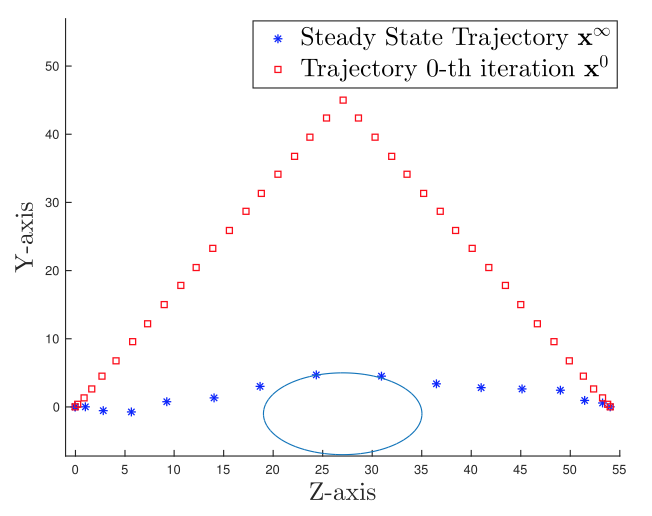
\includegraphics[width=.75\textwidth]{Screenshots for related work/Asset p2/Asset p2p1.png}}
\caption{SS positions over ZY plane
\cite{rosolia2018a}}
\label{fig:p2p1}
\end{figure}

\section{Applications for Data-Driven control }

Article \cite{bu2018a} analyzes the behavior of data-driven control in the extreme case of output saturation. This paper also uses a linear system approximation approach with dynamic linearization, but also applies assumption that the system has an output saturation. This does increase the tracking performance but decreases the resting time of the closed loop system. 

Article \cite{pravallika2021a} is an official MATLAB tutorial to DDC, which we follow with our designed controller simulation in the beginning of our project.

A recent article \cite{Berberich_2020} overviews a problem of state-feedback controllers for discrete-time linear time-invariant systems, based directly on measured data. This paper presents the robust methods for data-driven control in which the stable closed-loop performance is guaranteed even in presence of noise in data. The design of state-feedback controllers is based on the parametrization technique analyzed in \cite{de2019a}, particularly the application of robust control techniques to the parametrization, which results in stable performance of the closed loop control with noisy inputs.

\begin{figure} [h!]
\centerline{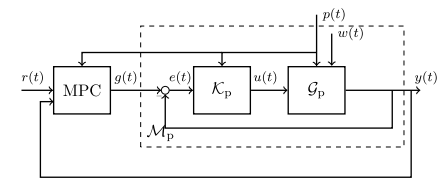
\includegraphics[width=.75\textwidth]{Screenshots for related work/constraint_data_driven_control_screenshot1.png}}
\caption{Proposed hierarchical control architecture
\cite{piga2017direct}}
\label{fig:hierarchicalcontroller}
\end{figure}

In the paper \cite{piga2017direct} a data-driven approach is used to design a hierarchical controller which includes the inner and outer controllers to enhance the overall performance of the inner controller. The evaluation of the effectiveness of this type of method is done by means of simulation and practical experiments. Basically this paper proposes the implementation of the outer Model Predictive controller used for improving the performance of an inner closed loop controller. In such a way it is not only improves the overall performance of the system, but also takes care of constraints imposed on inputs and outputs. Figure \ref{fig:hierarchicalcontroller} shows the resultant hierarchical controller, in which it can be seen that the outer Model Predictive controller tracks the input and output variables and operates on the reference signal applied to the inner loop in order to satisfy the constraints imposed on inputs and outputs of an overall system as well as improve on the system performance. To test the results the simulation of a servo positioning system in dc motor was used. The inner loop controller design resulted in the following performance shown in figure \ref{fig:hierarchicalcontroller}. However because of the lower degrees of freedom of the controller the controller could not obtain the faster dynamics and thus resulted in slow dynamics with the rise time of about 4 s. Adding the model predictive controller resulted in much better performance as shown in figure \ref{fig:hierarchicalcontroller}. The rise time resulted in 1.3 s, which is about 3 times as much faster as the previous result. 


A PhD thesis \cite{kergus} explores a Data-driven model reference control in the frequency-domain. 

An article \cite{CAMPESTRINI20172628} deals with Data-Driven (DD) control design in a Model Reference (MR) framework. 

Article \cite{vuillemin2019hybrid} shows a discrete-time control-law from frequency-data of a continuous-time plant so that their hybrid interconnection matches a given continuous-time reference model up to the Nyquist
frequency. 

Article \cite{Waarde2020} Data Informativity: A New Perspective on Data-Driven Analysis and Control explores the possible issues with data collected for data-driven control. Authors conclude that data-driven methods are capable of controller design in presense of much less data, when compared to system identification methods.

\begin{figure}
\centerline{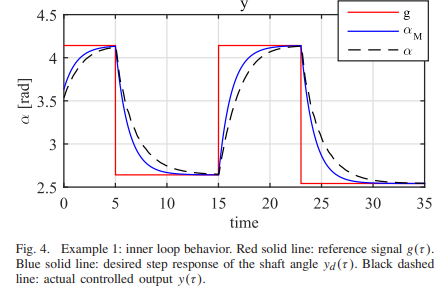
\includegraphics[width=.49\textwidth]{Screenshots for related work/constraint_data_driven_control_screenshot2_innerloop.png}
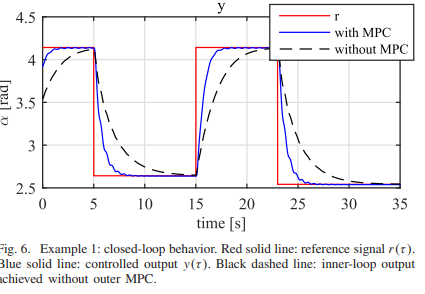
\includegraphics[width=.49\textwidth]{Screenshots for related work/constraint_data_driven_control_screenshot2_usingMPC.png}}
\caption{(a) Inner loop behaviour (b) and Closed loop behaviour with added MPC 
\cite{piga2017direct}}
\label{fig:pidcomparison}
\end{figure}

Overall, it could be concluded that Data-Driven control is becoming the primary focus of the control theory research, as more data and processing powers are available to researchers. This could be noticed by comparing the number of research papers published on the topic for the last years: the amount of publications has tripled since 2015 and the rate of new work on the topic continues rising. The review of related work has acquaint us with such import algorithms as NARX and DeePC, as well as MATLAB's System Identification toolbox and the Signal Builder.







\chapter{Experiment design and MATLAB simulation}

There are two main approaches considered: simulation and hardware implementation. In simulation part the DC motor model obtained from MATLAB Simscape toolbox was used as a plant model, whereas the hardware implementation was based on the simple DC motor of unknown model powered by driver and Arduino. The simulation part is considered to be the experiment design itself, as all of the required steps were first completed in the simulation. This chapter presents the taken steps for the experiment simulation in MATLAB.

\section{Data generation and collection}
The simulink model of a DC motor obtained from the Simscape toolbox is shown in figure \ref{fig:MatlabMotorModelAT1}, which is then used to log the input and output data in the setup described in figure \ref{fig:MatlabMotorModel}. The default Motor values were used for the first experiment, and later were modified to match those of a real motor to compare the modeled and hardware performance. The signal generator block was used to generate the input signals. Such a setup where the input and output are collected as applied voltage and motor speed is motivated by the desire to check the ability of data-driven control technique to adapt to various models. 

\begin{figure} [h!]
\centerline{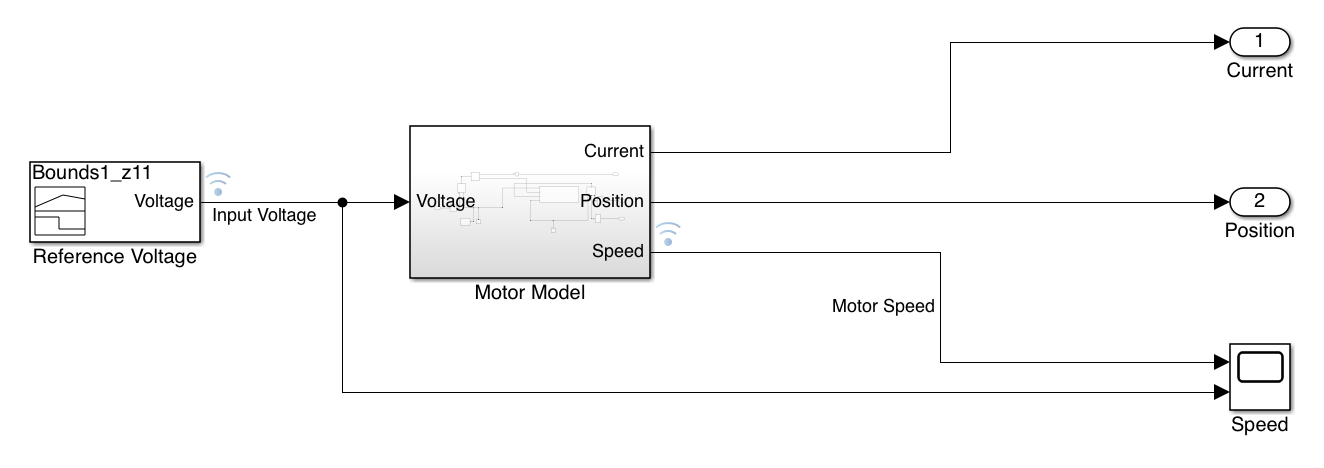
\includegraphics[width=.85\textwidth]{Screenshots for paper/matlab models/data aq model.png}}
\caption{MATLAB model for workspace data acquisition Simulink model}
\label{fig:MatlabMotorModelAT1}
\end{figure}

\begin{figure} [h!]
\centerline{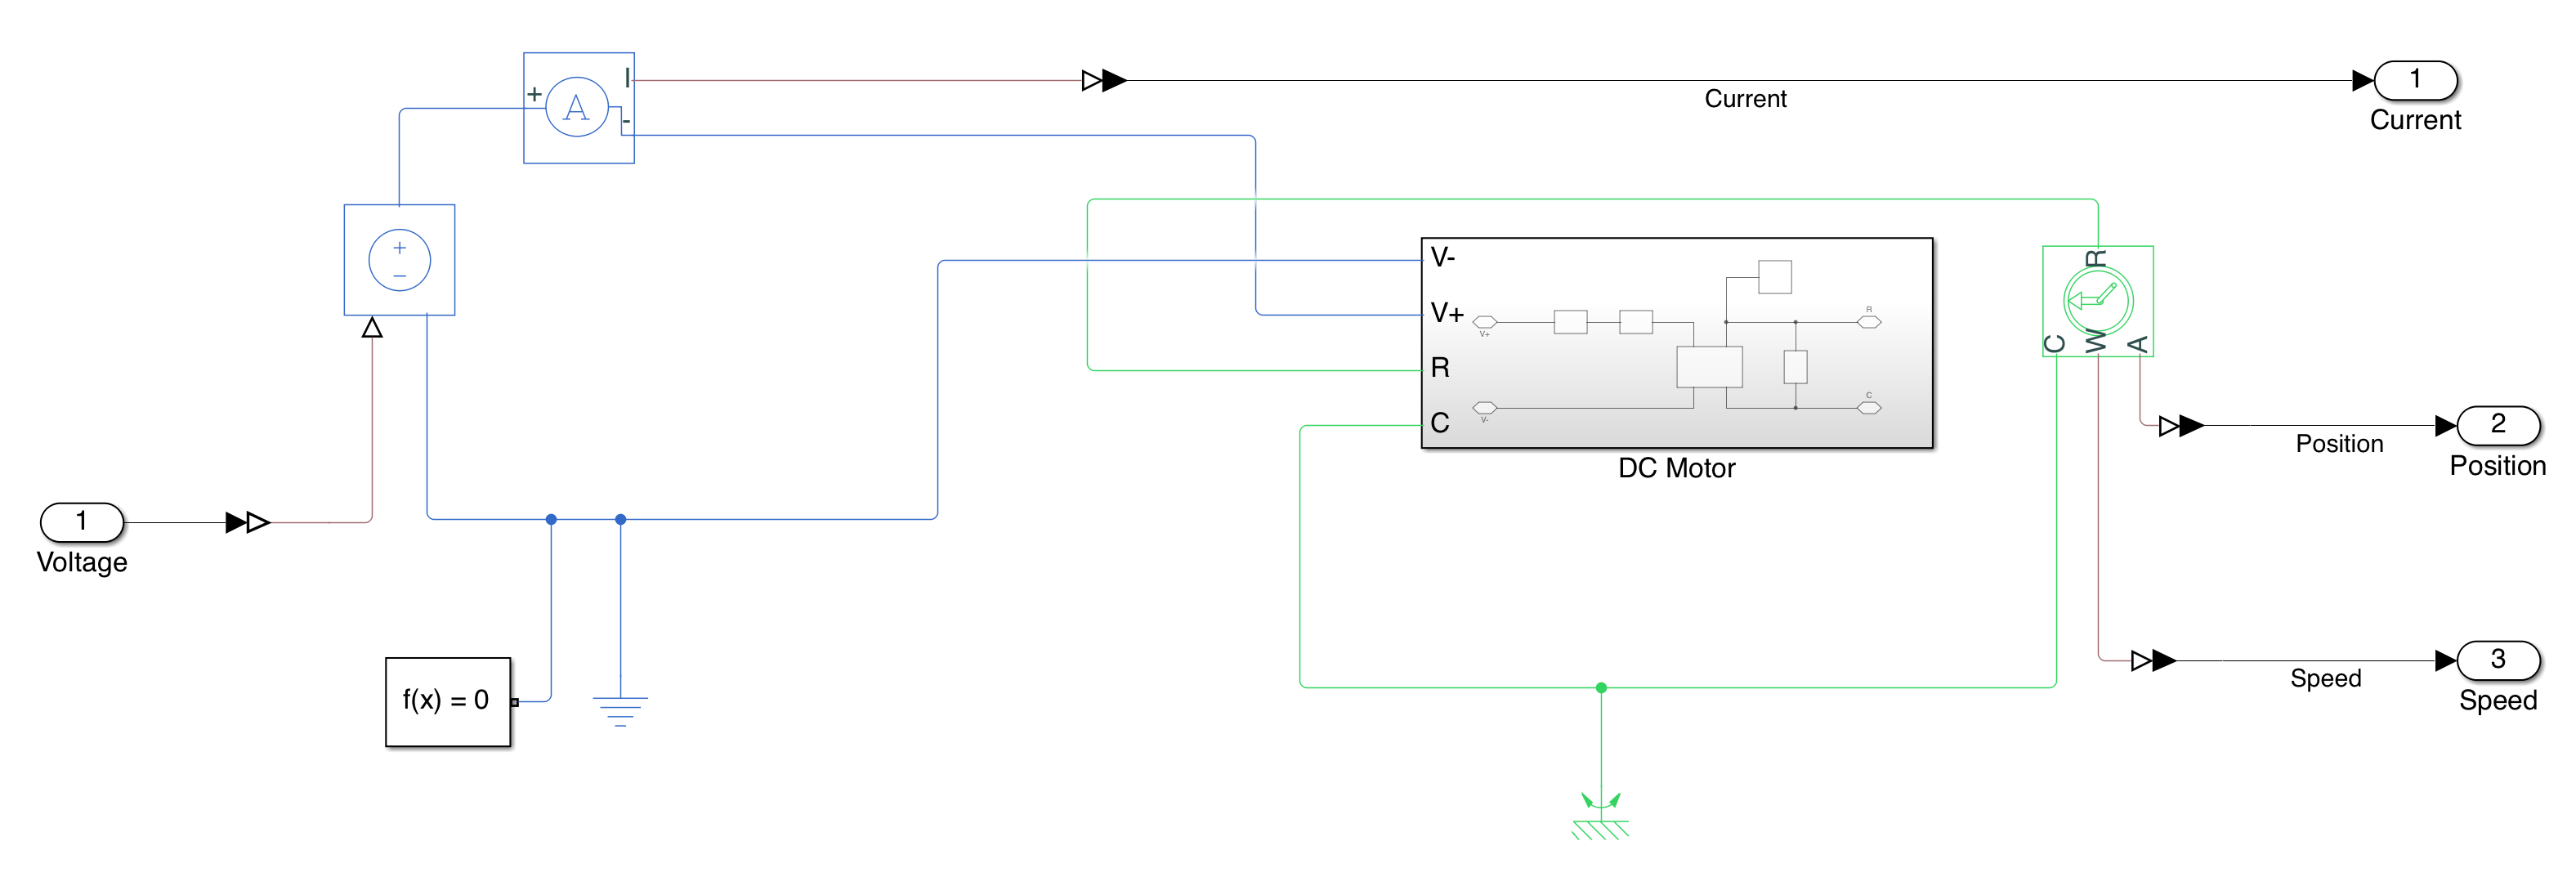
\includegraphics[width=.85\textwidth]{Screenshots for paper/matlab models/Motor Model.png}}
\caption{MATLAB Simulink Motor Model}
\label{fig:MatlabMotorModel}
\end{figure}

The signal generator used in this setup contained twelve signals of various shapes in order to capture the model dynamics as much as possible. Example of the process could be seen in Fig. \ref{fig:dataexp}.The voltage input to the DC motor is on the bottom graph and the motor position on top.

\begin{figure} [h!]
\centerline{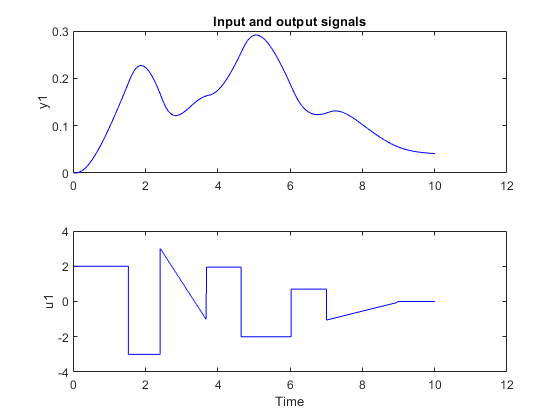
\includegraphics[width=.75\textwidth]{Screenshots for paper/matlab models/training_dataset_simulation.png}}
\caption{One of data collection experiments: voltage input to the DC motor is on the bottom graph and the motor position on top.}
\label{fig:dataexp}
\end{figure}

All of 12 experiments were then concatenated to a single input-output signal file for further processing.

\section{Model identification}
The model identification step could either be very detailed, long and thus computationally expensive, or it could be done based solely on the required dynamics of the model we are working on. While the first approach has its advantages and has a possible application scenarios (for example in space exploration), we are working on a simpler and faster solution. Thus, the model identification was implemented using the system identification app in MATLAB. The continuous-time transfer function was created based on the acquired data with linear behaviour experiments. Also, NLARX was used for the nonlinear system identification based on the nonlinear experiments (i.e. sine function and other variants). In further experiments, the values for the real, known DC motors were substituted in the simulation model and the resultant transfer function was compared with that of real one.

\section{PID Controller design}

\begin{figure} [h!]
\centerline{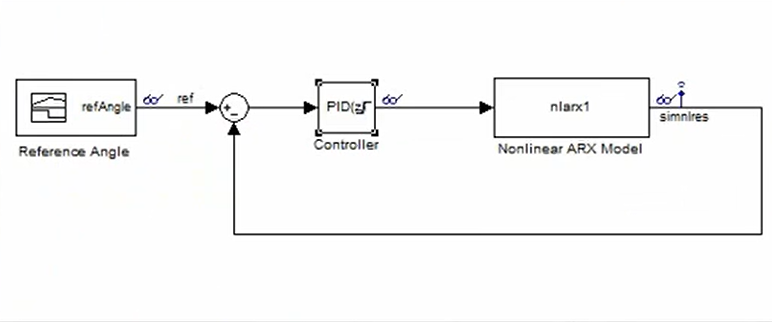
\includegraphics[width=.85\textwidth]{Screenshots for paper/matlab models/PIDdesign.png}}
\caption{MATLAB model for the PID controller design based on the identified model}
\label{fig:PIDdes}
\end{figure}

The controller is designed using PID tuner toolbox in a simple setup shown in Fig. \ref{fig:PIDdes}. The Simulink model obtained in previous step is linearized in this step and the controller gains are adjusted accordingly. This step provides an ability to adjust the needed controller characteristics, for example prioritize overshoot removal or decrease the response time. The balance is important in those settings as it provides optimal behaviour accuracy. The designed controller is then tested.


\begin{figure} [h!]
\centerline{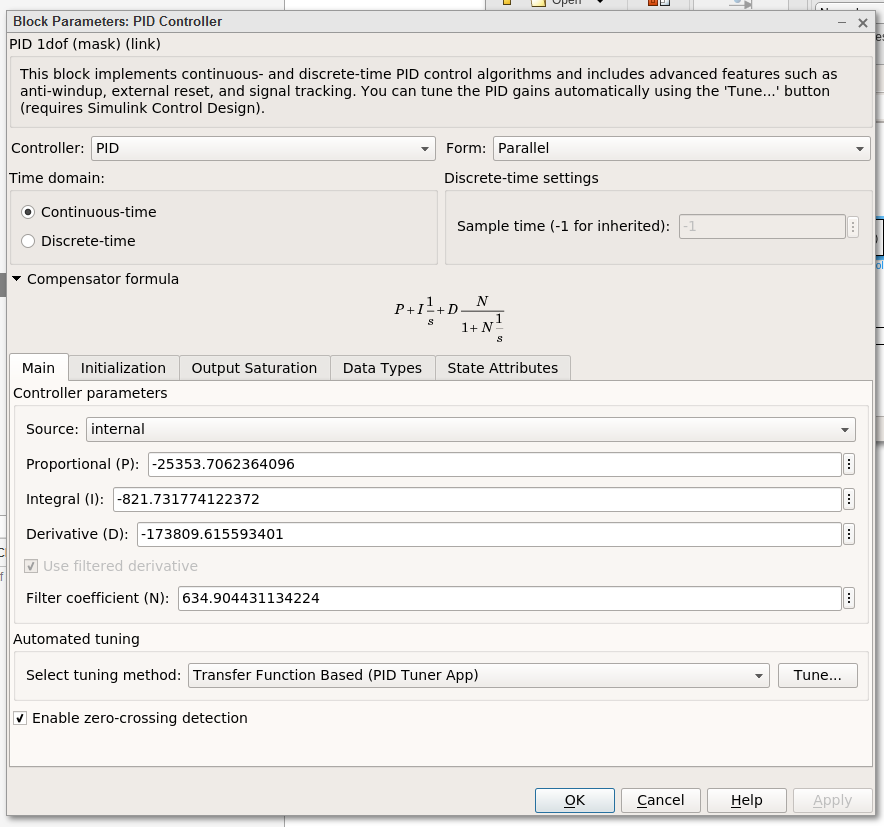
\includegraphics[width=.85\textwidth]{Screenshots for paper/arduino/Final_hardware_testing/pid_tuner.PNG}}
\caption{PID controller designer}
\label{fig:PIDtunerMATLAB}
\end{figure}

The main advantage is obvious. The MATLAB has a lot of useful tools to tune and check the dynamic systems and filters applied to them to see the bound conditions and instabilities before implementation. However, that does introduce some unknown variables and concepts that were did not anticipate to use. The best example of such complications is Compensator formula from the PID controller simulink block parameters, which has a Filter Coefficient that is not typically present in the PID micro-controller devices.




\section{Testing}

Testing is done by supplying a voltage signal to the above mentioned model (Fig. \ref{fig:PIDdes} with designed controller and tracking the output (DC motor position). 

Further tests include the modification characteristics of DC motor model to match those of a real DC motor and compare the performance of the experiment design. The used DC motor model could be seen in Fig. \ref{fig:MatlabMotorDCpart}. 

\begin{figure} [h!]
\centerline{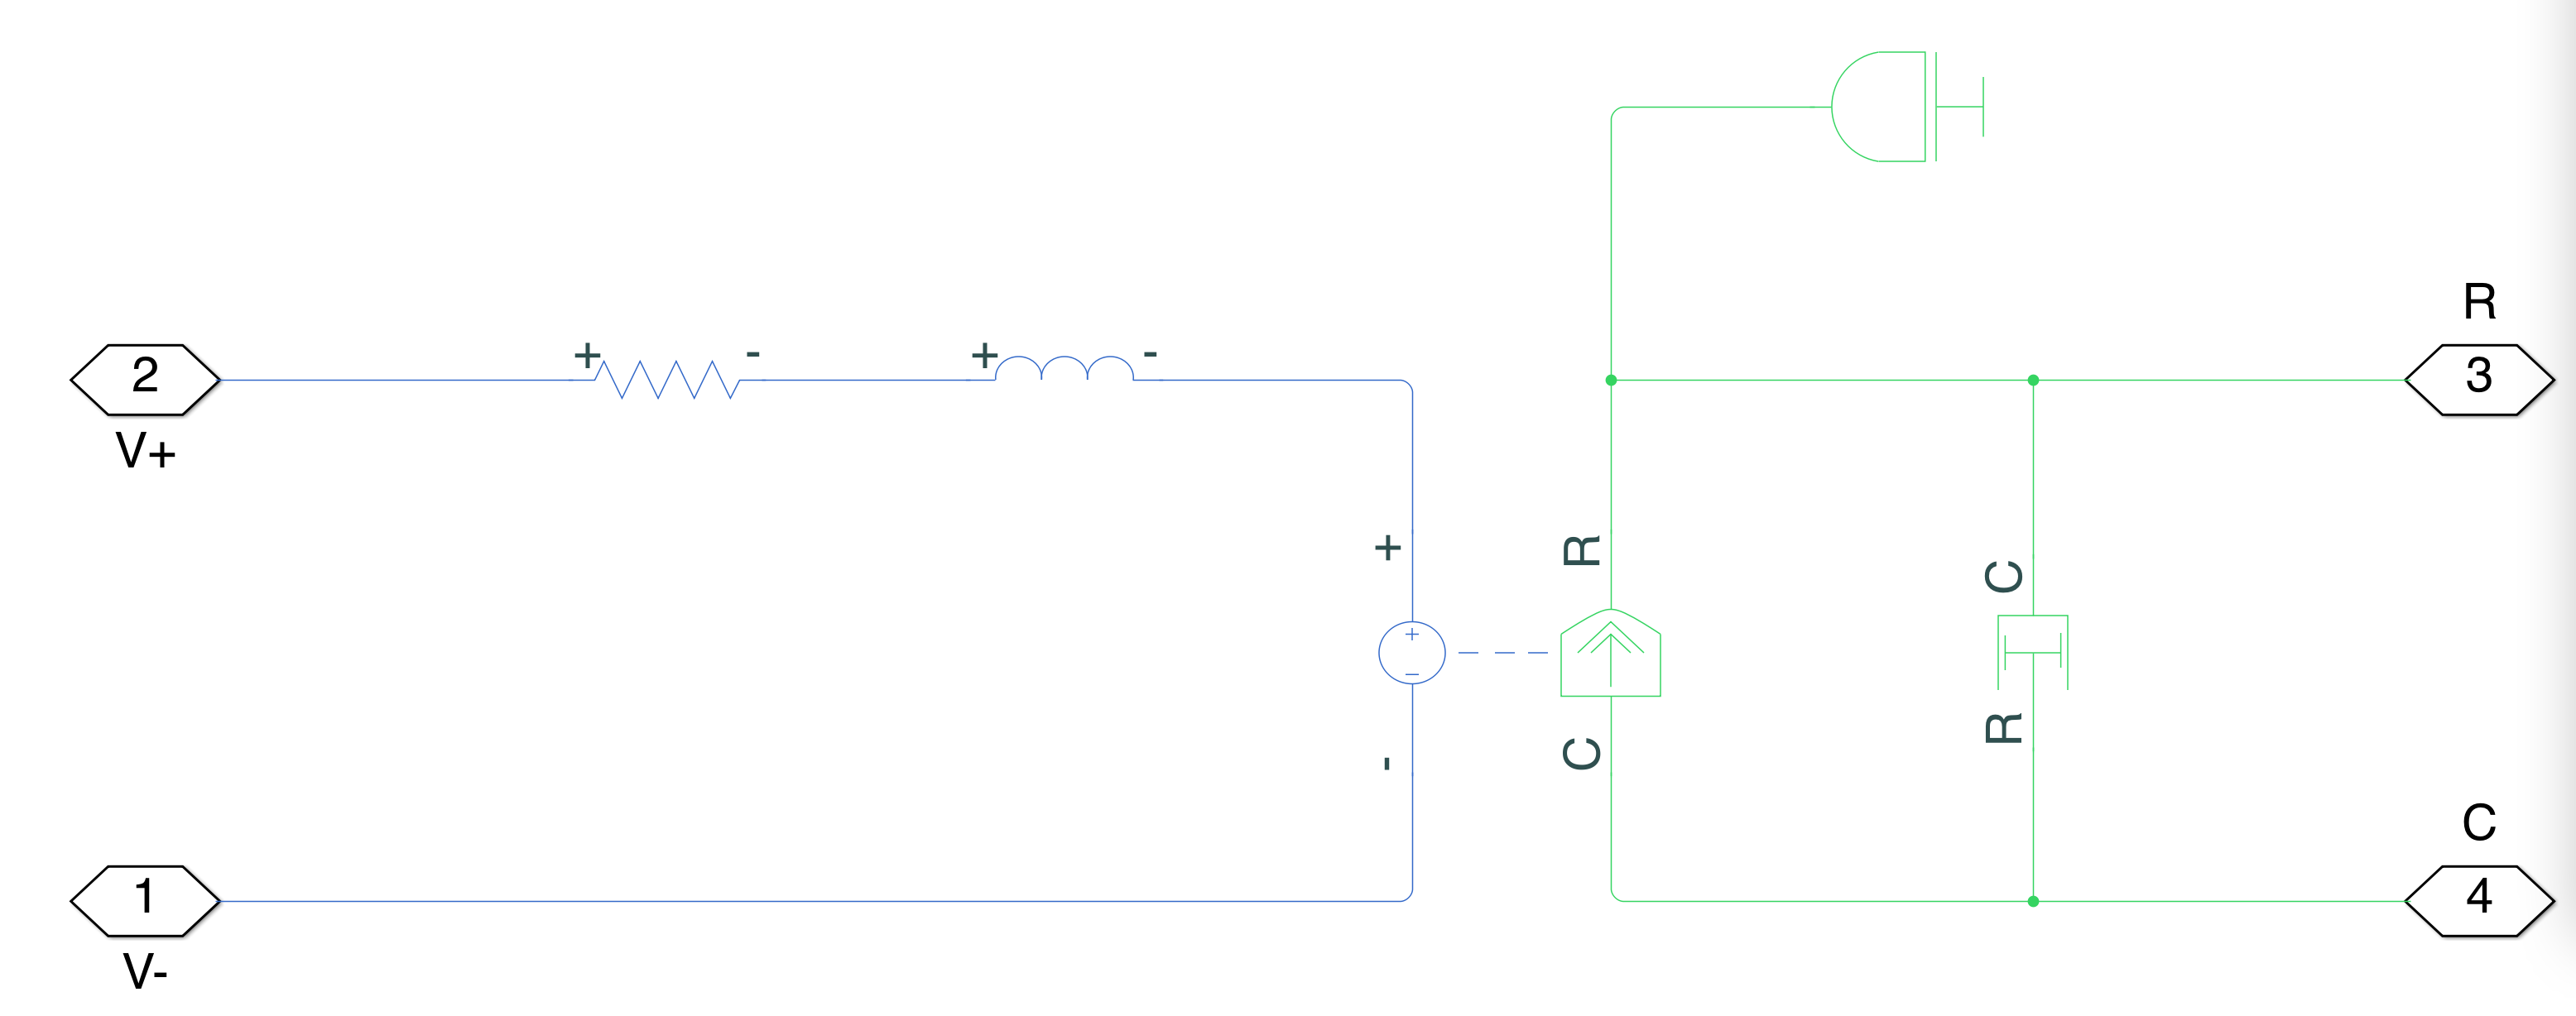
\includegraphics[width=.95\textwidth]{Screenshots for paper/matlab models/DC Motor.png}}
\caption{MATLAB Simulink DC Motor isolated part}
\label{fig:MatlabMotorDCpart}
\end{figure}



\chapter{Hardware Implementation}

\section{Arduino}

\begin{figure} [h!]
\centerline{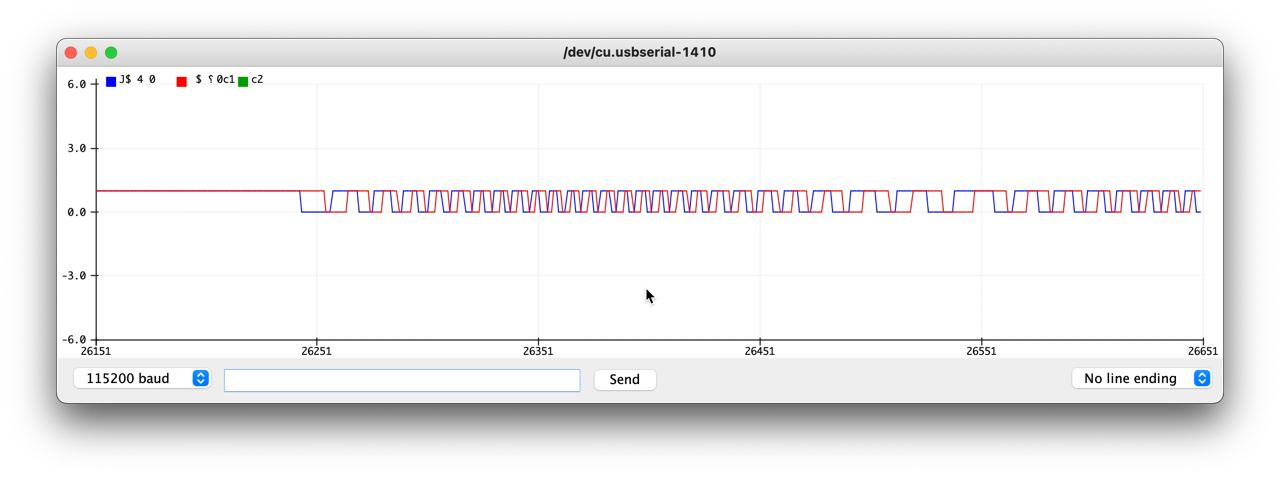
\includegraphics[width=.95\textwidth]{Screenshots for paper/arduino/encoder signal.jpeg}}
\caption{Arduino plot for encoder signal}
\label{fig:arduinoEncoder}
\end{figure}

Arduino IDE is a software environment that creates near native machine code with included Arduino.h header. Figure \ref{fig:arduinoEncoder} shows the incoder signal plotted using Arduino.h's digital read and Serial plot libraries. The signal is produced by rotating rotor with encoder by hand. This might be important because even thought signal looks great, it is plotted on low angular velocity.

\begin{figure} [h!]
\centerline{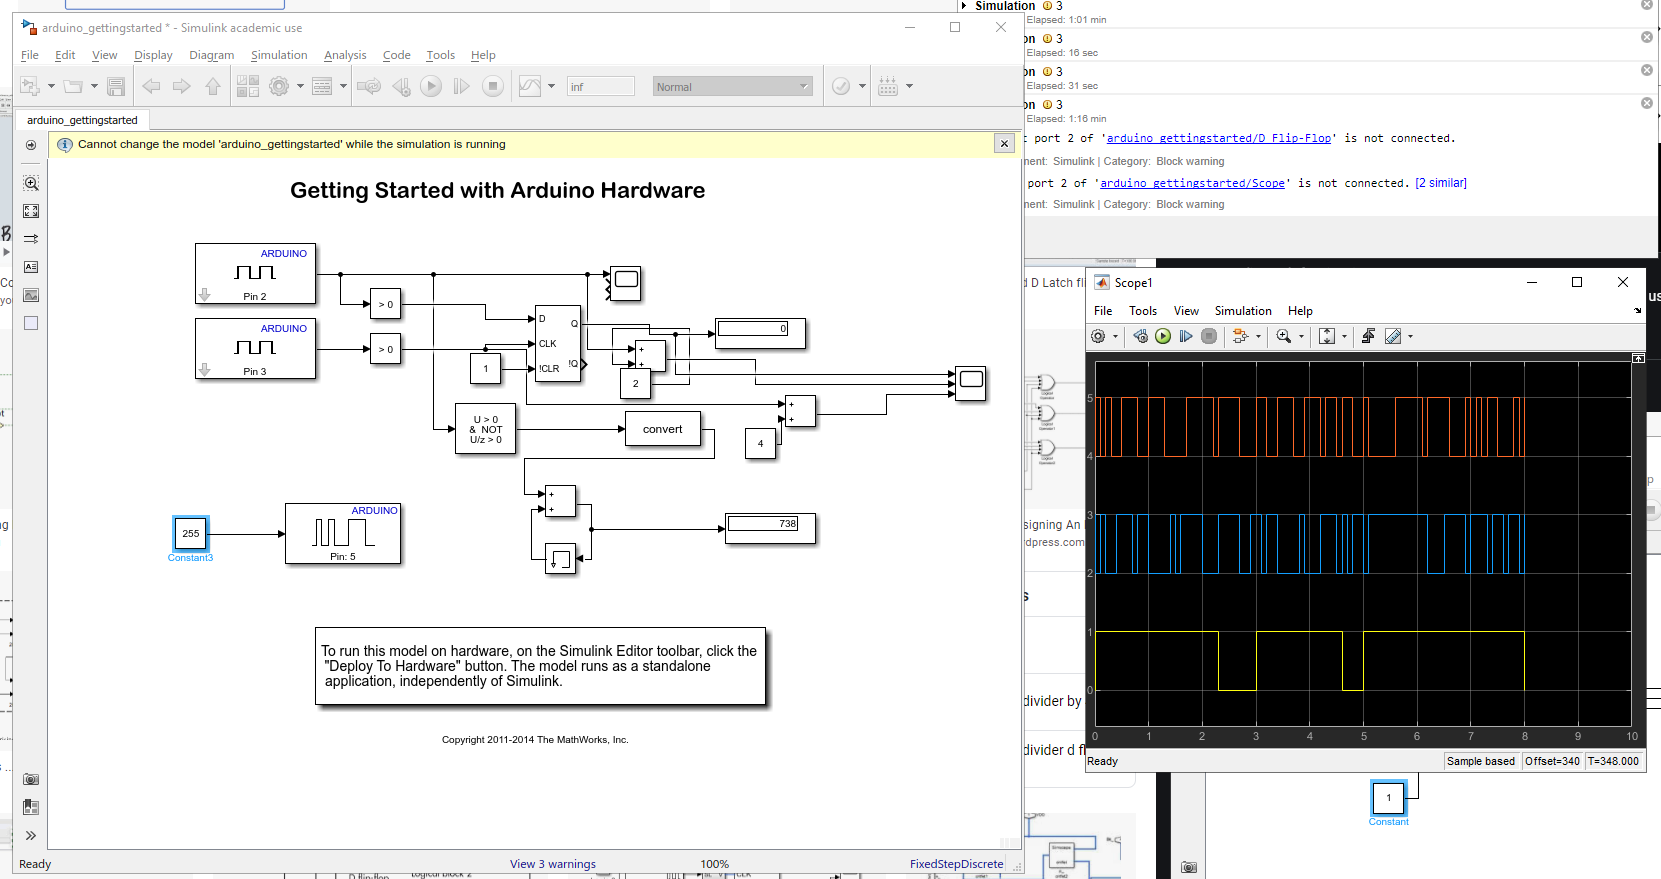
\includegraphics[width=.95\textwidth]{Screenshots for paper/arduino/Model encoder arduin MATLAB.PNG}}
\caption{MATLAB Simulink Arduino model}
\label{fig:arduinoSimulink}
\end{figure}

Comparing to a traditional Arduino programming, MATLAB does not provide low level hardware access into the registers and peripherals of the board. Instead it is given as abstract Simulink model blocks with predefined clock and settings.

\begin{figure} [h!]
\centerline{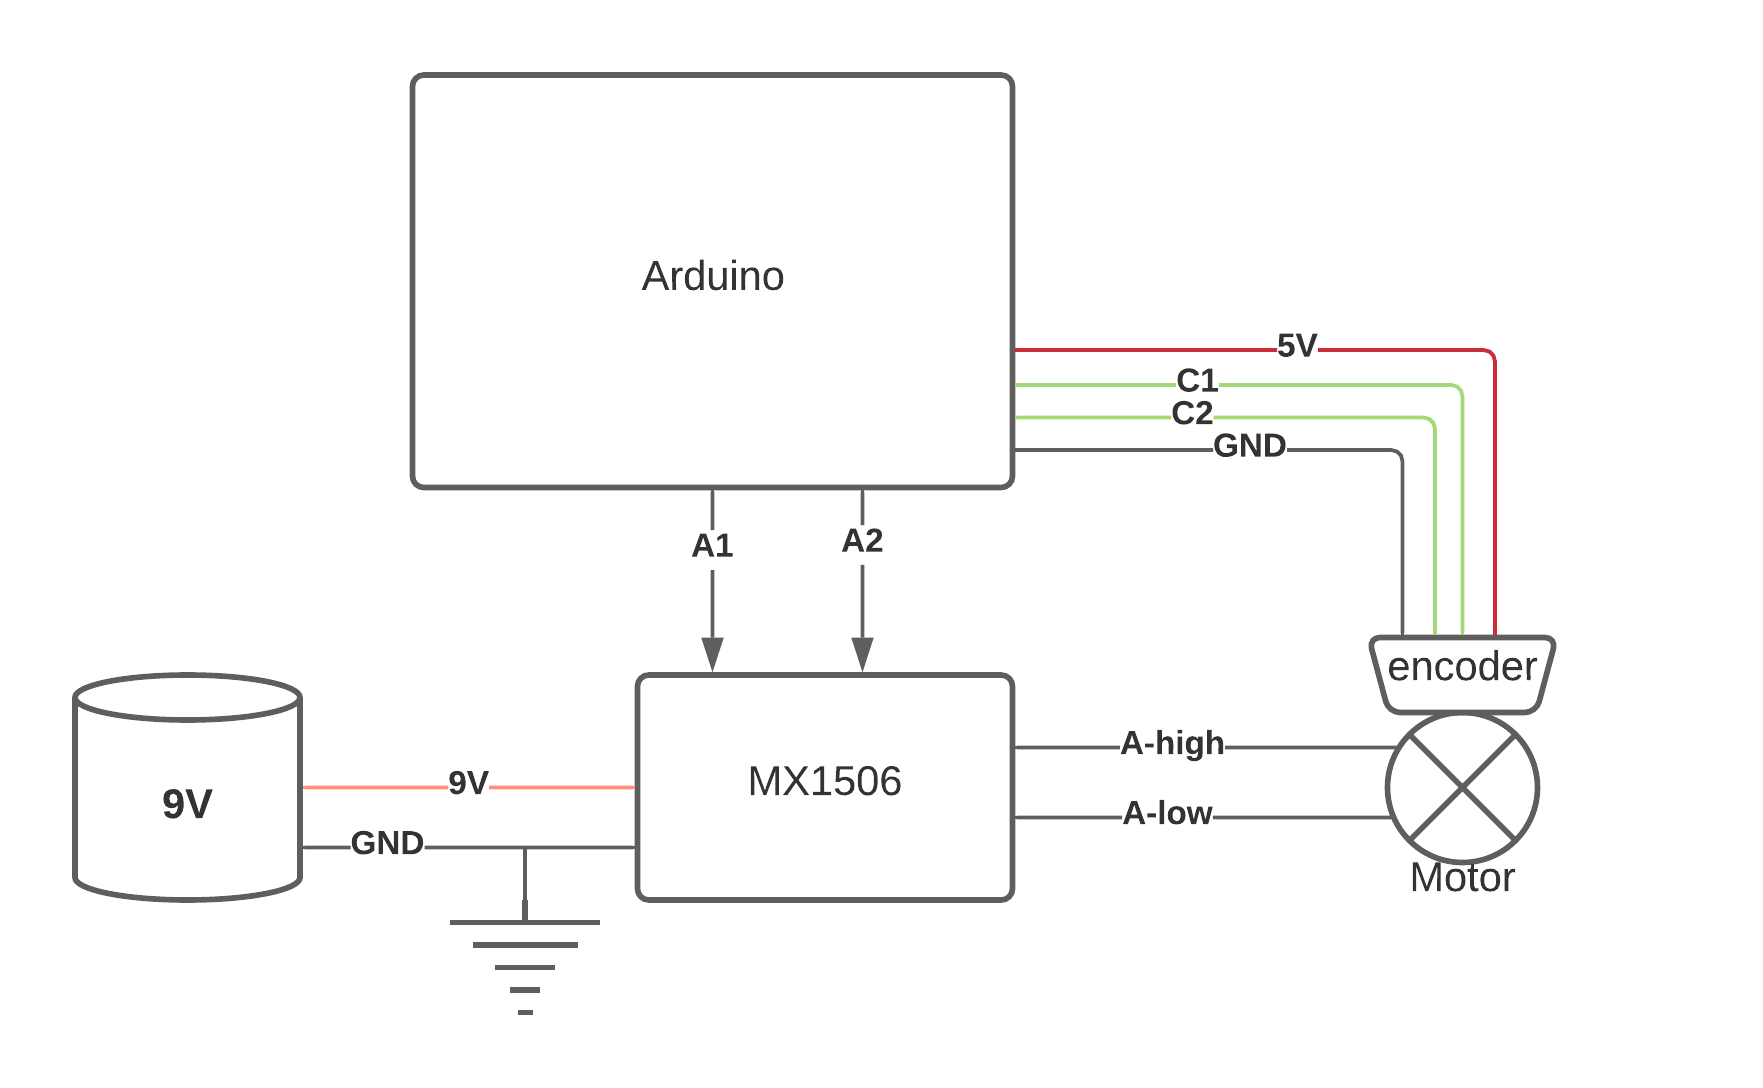
\includegraphics[width=.75\textwidth]{Screenshots for paper/arduino/model1/dc motor model1.png}}
\caption{Arduino motor hardware setup diagram}
\label{fig:arduinoMotorSetupDiagram}
\end{figure}

The Arduino MATLAB hardware setup consists from three major parts: a DC motor, Arduino compatible board (Arduino UNO R3), Encoder. The motor is driven by an external motor driver board. The exact board used is a simple no brand model based on MX1508 chip that also would require external fly-back diodes to operate in more safe conditions, but we have omitted them due to low power nature of chosen motor and just prayed God that we would not fry our personal computers or lab equipment. The driven board seems to have no dedicated ground for the signal wires, which is a bit worrying. We did nothing about it, but could just have shared power ground. The MX1508 is a simple and cheap dual channel (A and B) motor driver that can drive up to 2 amperes of current on a voltage range of 2 to 9.6V nominal. we have hooked it up to common 9V alkaline battery, again due to low power nature of the motor, it was believed that this battery will suffice, use more power full power supply otherwise. The motor that we used came with built-in encoder that has two power and two signal terminals that provide variable frequency square wave signal with a phase shift of quarter cycle. This type of encoders are easy to read and can provide both direction and angular velocity of the motor.  

\begin{figure} [h!]
\centerline{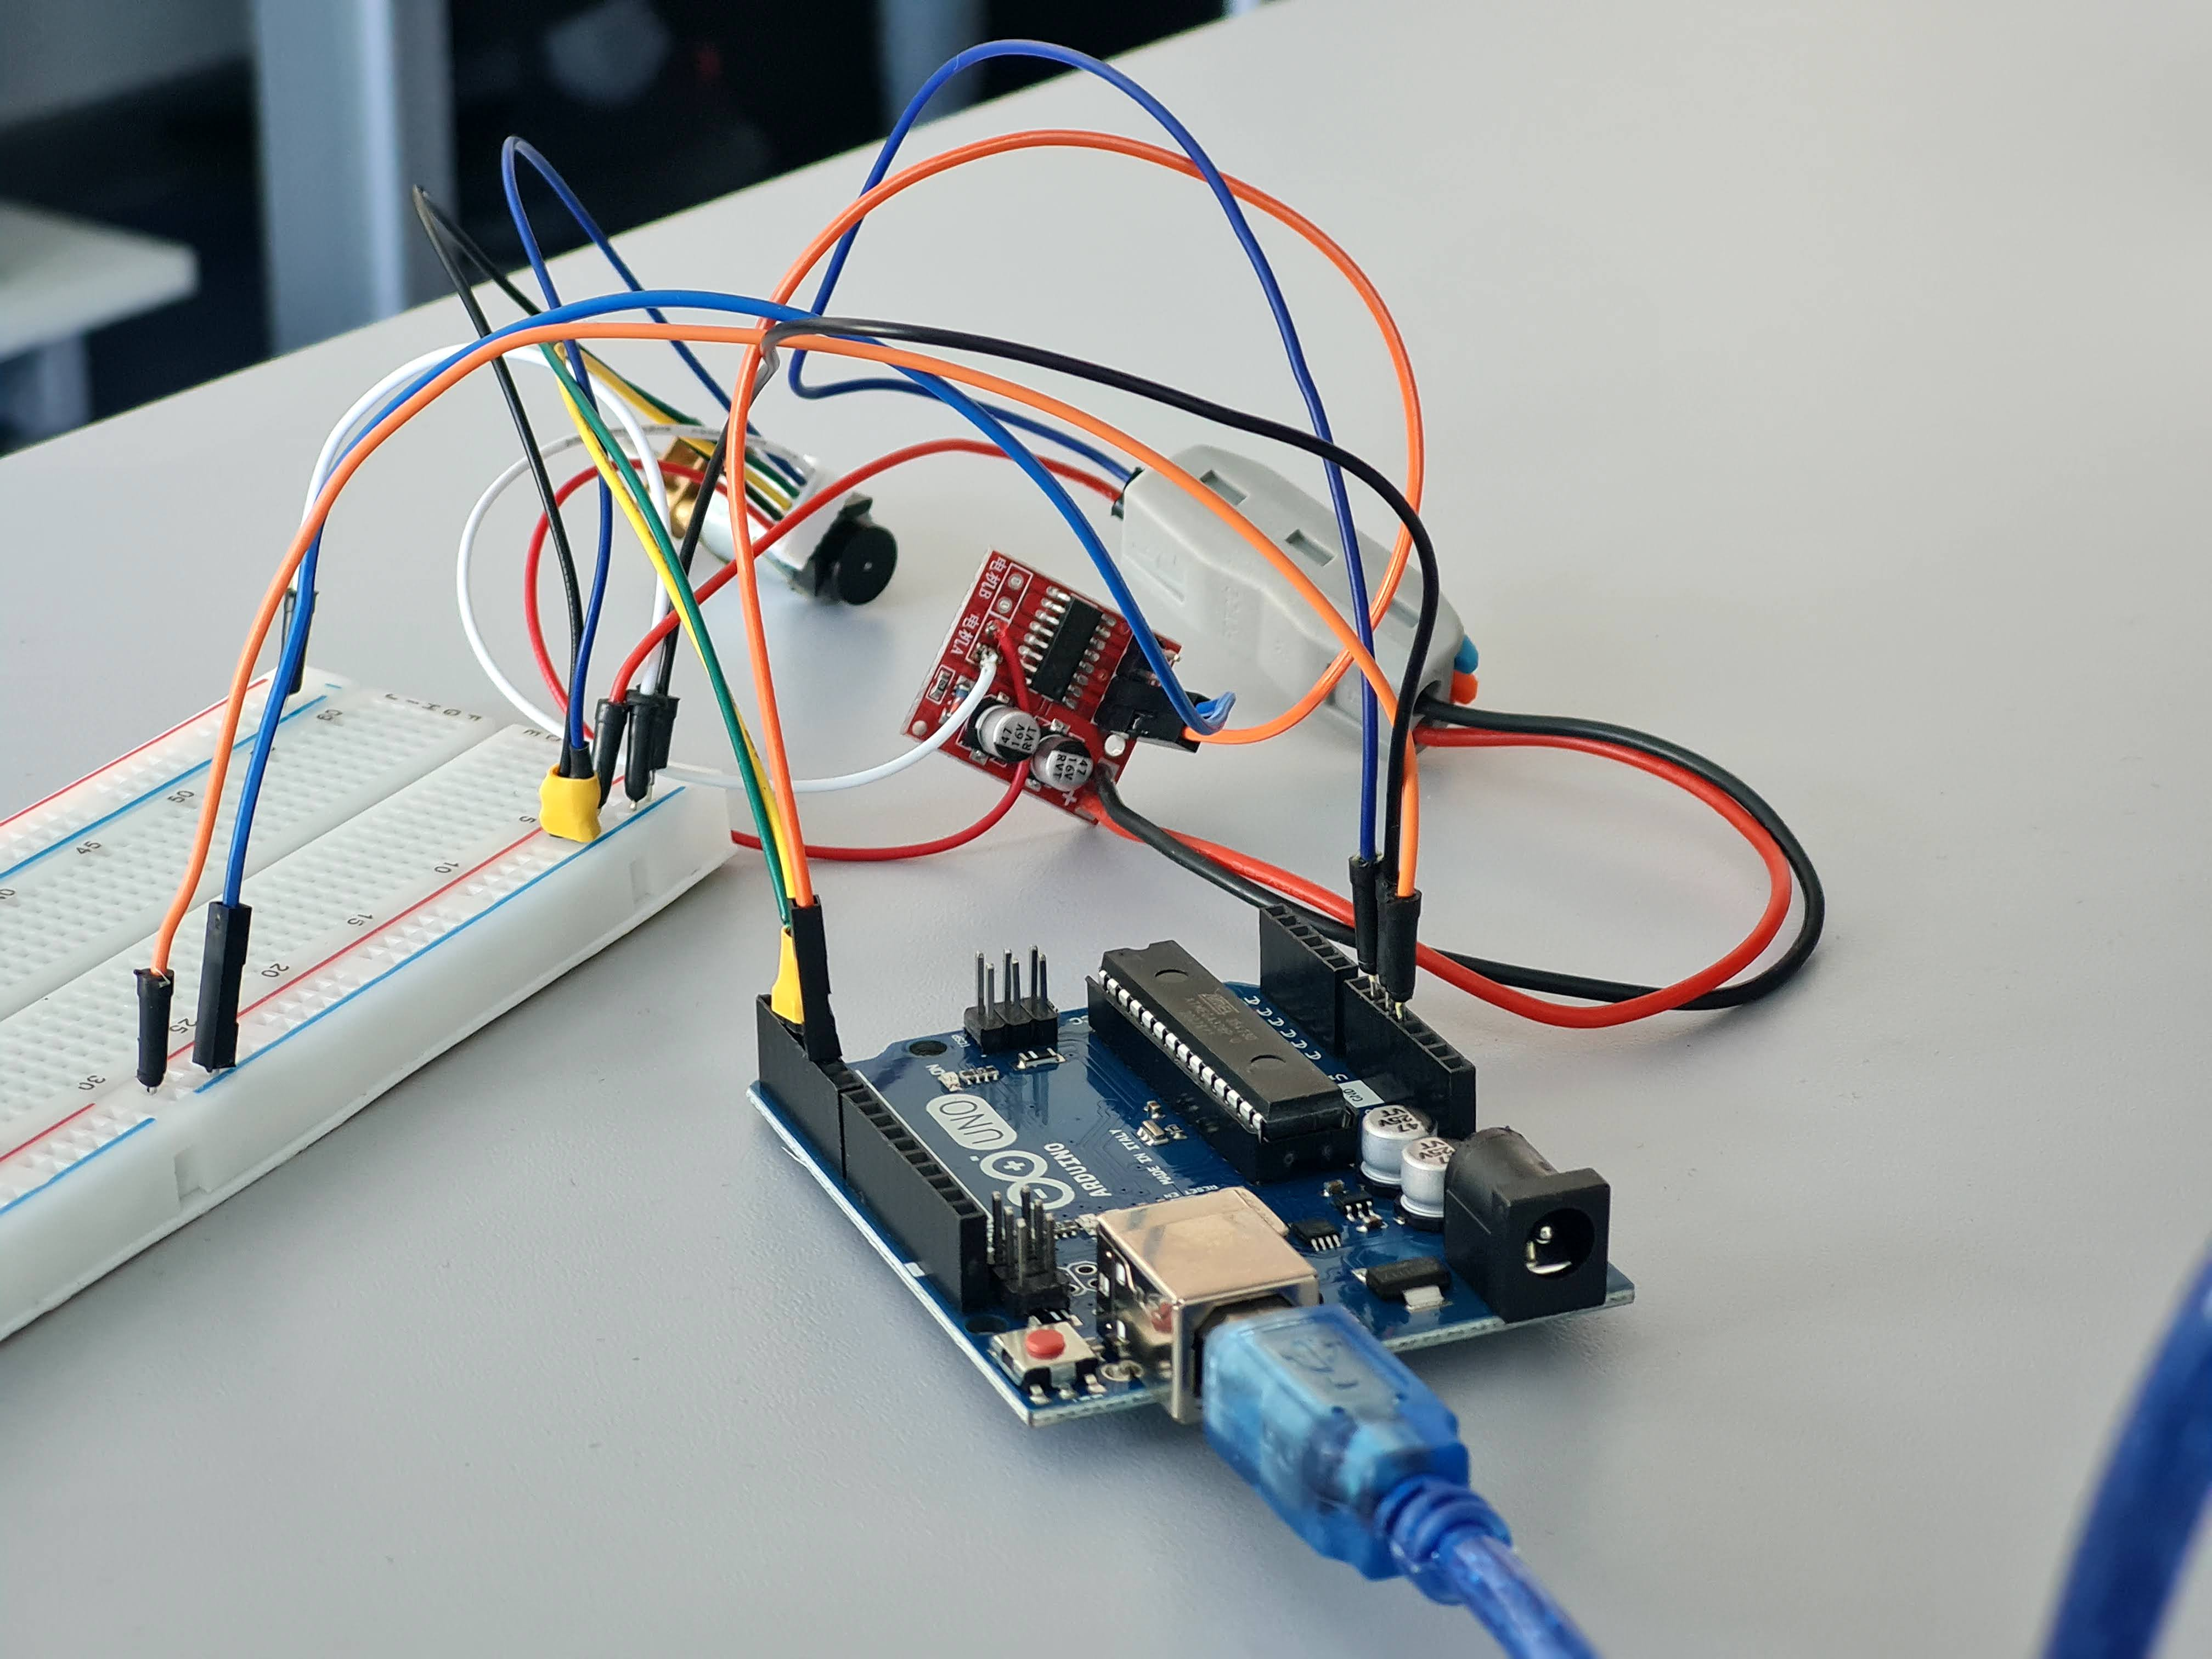
\includegraphics[width=.75\textwidth]{Screenshots for paper/arduino/arduino motor setup 1.jpg}}
\caption{Arduino motor hardware setup}
\label{fig:arduinoMotorSetup}
\end{figure}

After checking encoder signal we assembled a MATLAB Simulink \ref{fig:arduinoSimulink} model to be able to read encoder's speed and direction. This time rotor was driven by applied voltage on the motor. This way we got stable uniform encoder signal to check the encoder velocity units and direction. We were partially successful. Quick observation shows that even though the motor had constant velocity with no load or oscillations on direction the model showed chaotic alternation in motor direction. After analysing the recorded signal we come to the conclusion that model with Arduino could not keep up with the signal and the samples resulted in aliasing. This was further proven when we tried to increase the sample frequency of the Arduino simulink model. There is a possibility that there is some additional sample rate related parameters of the model that could solve problem with aliasing, but we did not find it and came to a conclusion that Arduino's MATLAB Simulink implementation is just simply not fast enough. There could be made a walk-around by coding the Arduino with its native Arduino IDE to minimize the overhead and set up custom bare minimum communication method over virtual com port UART.


\subsection{Commercial servo motor setup}

\begin{figure} [h!]
\centerline{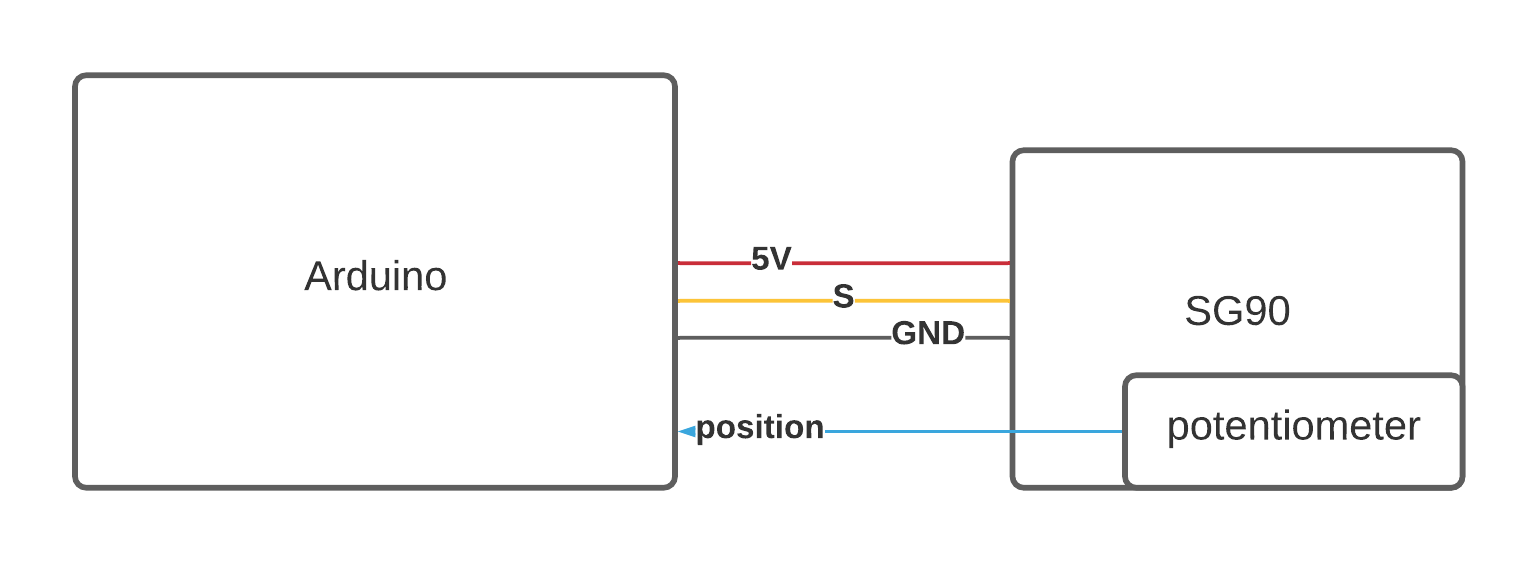
\includegraphics[width=.75\textwidth]{Screenshots for paper/arduino/model 2/model2.png}}
\caption{Arduino with Commercial servo motor setup}
\label{fig:arduinoMotorSetupDiag2}
\end{figure}

After we initially have failed to read the encoder's positional data from Arduino using MATLAB we have decided to try to use another type of motor \ref{fig:arduinoMotorSetupDiag2}. Even thought it is still essentially simple DC motor, it has a high rate gears and feedback potentiometer. Typically this type of servo motors are used as open loop controllers with no feedback what so ever. But we decidede to open it up and solder Arduino's internal analog to digital converter right on the middle terminal of the potentiometer.

\subsection{Speeding things up}

It is possible to use previously metioned MATLAB + Arduino method even thought we could not keep up with the reading from encoder. The trick is to use two separate Arduino's. First should be as usual connected to the MATLAB directly, but the second is configured to have external hardware interrupt pins to fire counter and check the position of the encoder. By using more expensive STM32F302R8C6 we have reached redundant and reliable source of ADC data and serial communication. 

\begin{figure} [h!]
\centerline{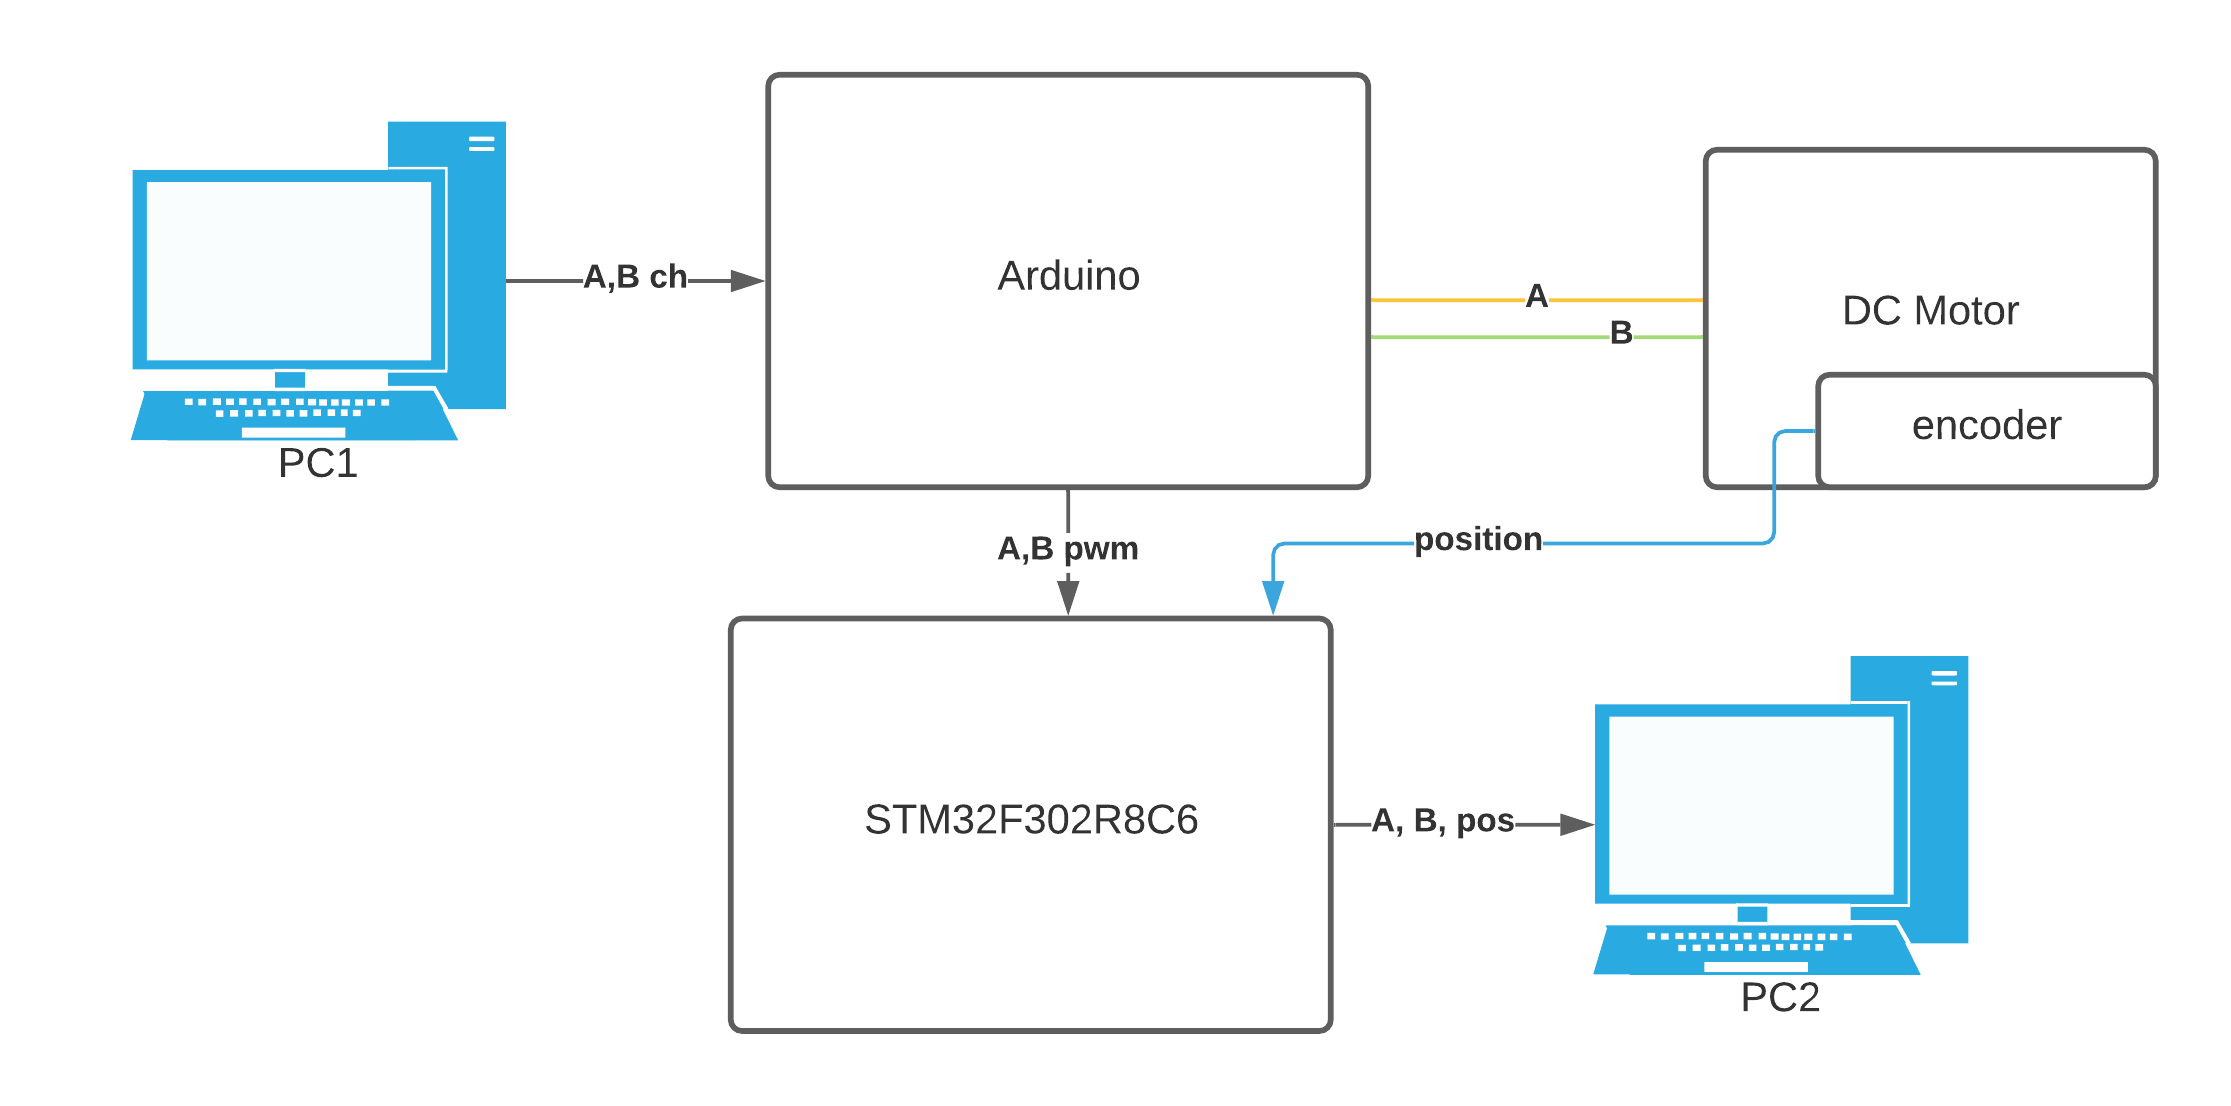
\includegraphics[width=.95\textwidth]{Screenshots for paper/STM32/Blank diagram.png}}
\caption{STM32 hardware setup model (model4)}
\label{fig:stm32f3_m1}
\end{figure}

In the \ref{fig:stm32f3_m1} diagram the PC1 is using MATLAB software and communicates with the Arduino UNO directly over UART and is in control of the motor signal. We have chosen STM32F3 as a substitute for another Arduino board due to its high clock (72Mhz over 8Mhz) and higher precision ADC (of 12bit) but is proven to be redundant. 

\begin{figure} [h!]
\centerline{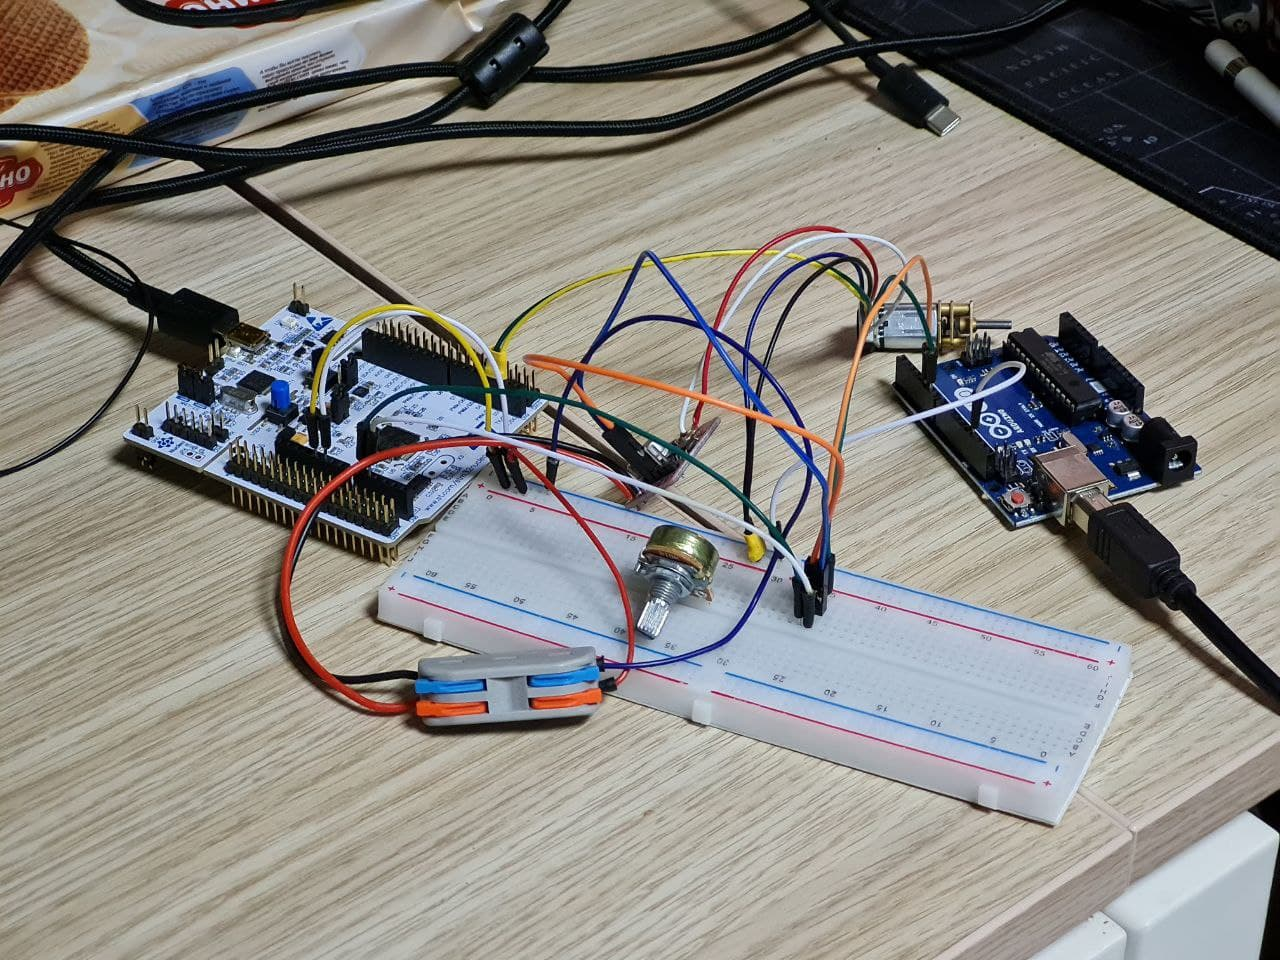
\includegraphics[width=.75\textwidth]{Screenshots for paper/arduino/model 2/setup2.jpg}}
\caption{Arduino with hardware setup model (model2)}
\label{fig:arduinoMotorSetupDiag2}
\end{figure}

It might be possible to reduce number of micro controllers just to single STM32F3 due to its high potential. This would allow us to skip manual logging and importing step entirely, but requires dedicated research time to try and set it up. So far we did not configure it directly to the MATLAB even if nucleo-64 boards are proven to be very Arduino compatible, but are planning in future.

\subsection{System Identification and controller evaluation}
\subsubsection{Signal Processing}\

Using two micro controllers to control the motor and log the data was a huge success. However there was a new problem of data synchronization. Because STM32 is capable of continuous analog to digital conversion we could just log down the input from the MATLAB to the control board without much data loss and then low pass the data to fit the input. There is a chance that due to low pass filter's ability to shift the phase, we could be off in the phase and that could affect the quality of both linear and non-linear approximation models from the system identification toolkit of the MATLAB software.

\begin{figure} [h!]
\centerline{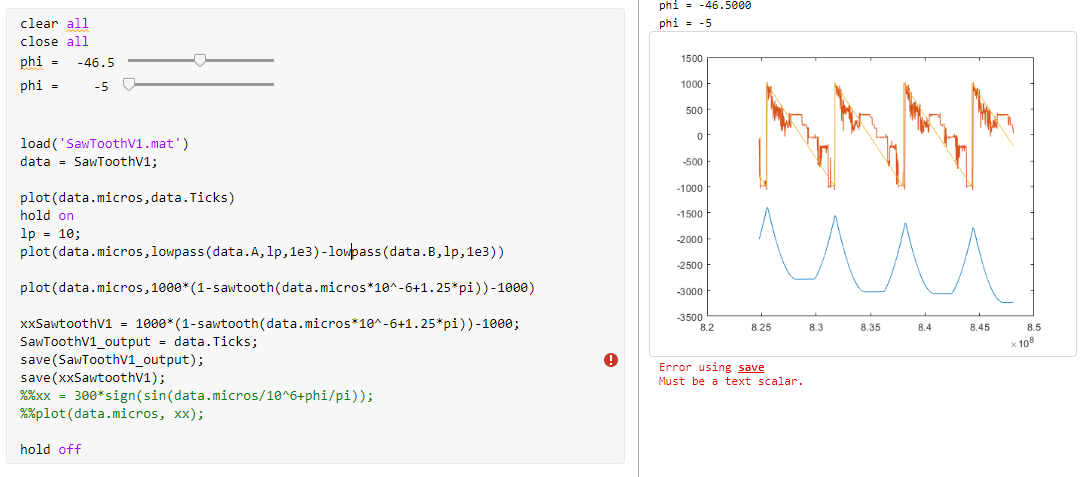
\includegraphics[width=.75\textwidth]{Screenshots for paper/matlab models/data reconstruction.PNG}}
\caption{logged data fitted to follow the input (low passed)}
\label{fig:dataReconstruction}
\end{figure}

The process of input logging, filtering and phase correction was applied for every signal sent to the system. This includes several seconds of multiple iterations on saw-tooth, square, sine and combination of those above motioned signals. Even though MATLAB's ability to identify the system is good. It does not fully utilize the hardware accelerations provided by our personal computers and does think for a while without noticeable load on both CPU and GPU. It is suggestible to have another software solution for system identification if possible due to inefficient use of computational resources.

\subsubsection{System identification results}
The obtained datasets were feed into system identification app for model generation.
Two models were obtained: linear transfer function and non-linear Auto Regressive with Exogenous input(NLARX) model. Below, figure \ref{fig:sysIdentfromSTMsetup} (a) represents the identified linear model representing in green, fitting the validation data by 41.07\%.  

\begin{figure} [h!]
\centerline{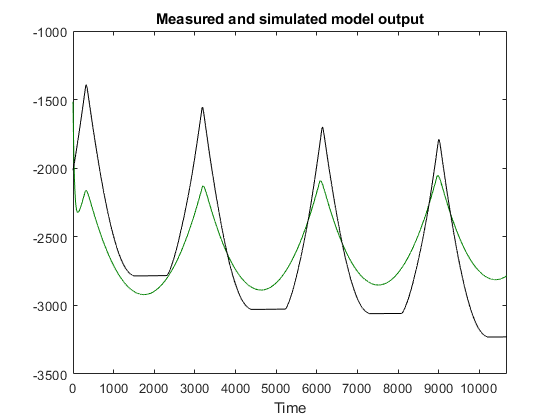
\includegraphics[width=.49\textwidth]{Screenshots for paper/arduino/tf_fixed_two_poles.png}
{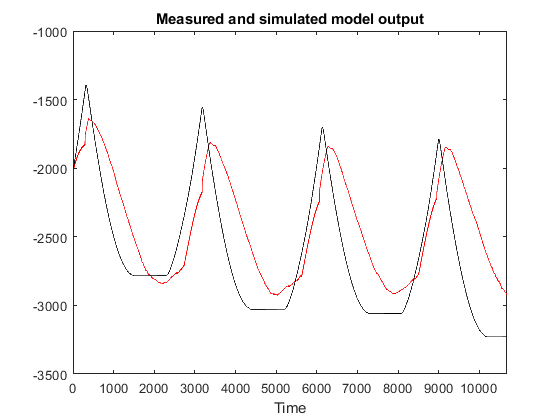
\includegraphics[width=.49\textwidth]{Screenshots for paper/arduino/nlarx_model_fit.png}}}
\caption{(a) Plot of the gathered and simulated output of the identified model over time (b) Plot of the gathered and simulated output of the identified nlarx model over time }
\label{fig:sysIdentfromSTMsetup}
\end{figure}


The nonlinear model shown in figure \ref{fig:sysIdentfromSTMsetup} (b) has resulted in about 20\% fit on validation dataset, which suggest that the training resulted in overfitting and the model can not properly fit the testing data. 


\subsubsection{Integrating linear model with PID controller}
The overall scheme is shown below in figure \ref{fig:arduinoSetupClosedLoop}

\begin{figure} [h!]
\centerline{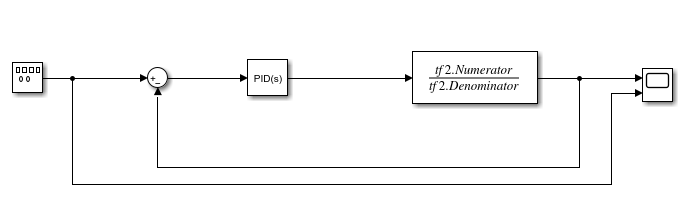
\includegraphics[width=.75\textwidth]{Screenshots for paper/arduino/Final_hardware_testing/closed_loop_linear.PNG}}
\caption{Closed loop with the linear model}
\label{fig:arduinoSetupClosedLoop}
\end{figure}

The result of feeding the setpoint sawtooth signal is shown in figure \ref{fig:Arduino_sawtooth}, with the controlled signal resulting in the following parameters: Rise time=21.3ms, Settling time=235ms.

\begin{figure} [h!]
\centerline{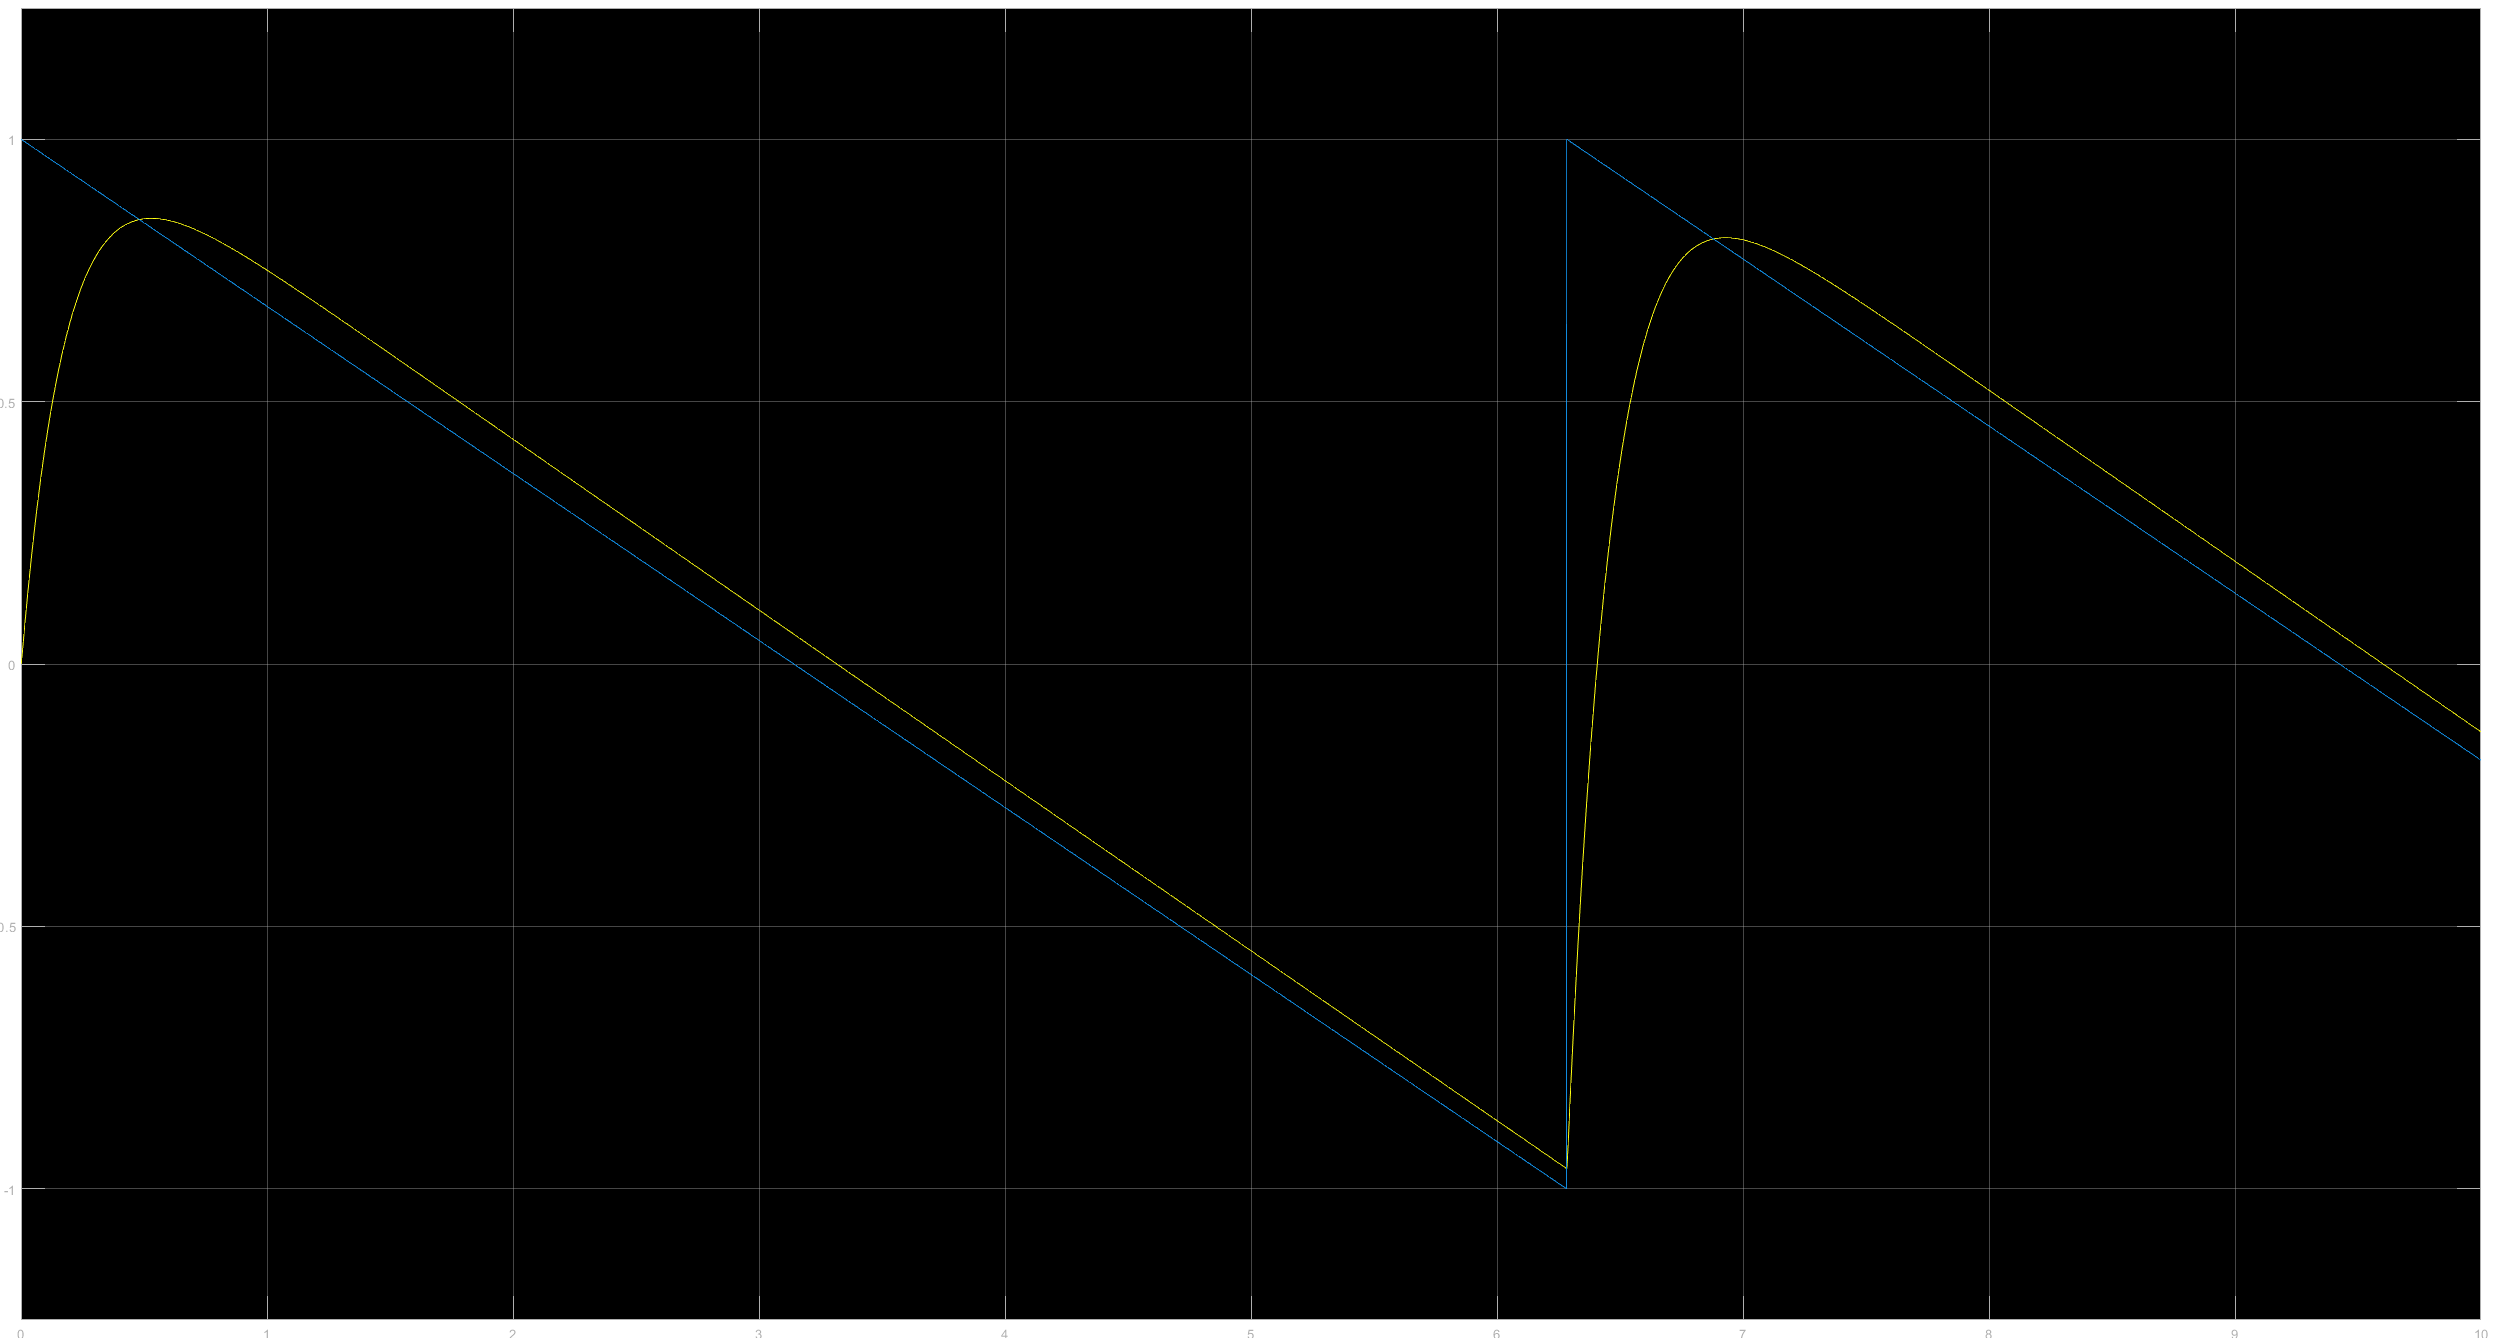
\includegraphics[width=.75\textwidth]{Screenshots for paper/arduino/Final_hardware_testing/sawtooth_response.png}}
\caption{Sawtooth signal}
\label{fig:Arduino_sawtooth}
\end{figure}

\section{dSpace}

The dSpace is a tool that comes as PCIe expansion card. The card is designed to be connected with external PCB inverter that runs the motor and ADC. It interfaces peripherals as MATLAB Simulink block that interfaces with motor simulation models. There is also a 3rd party monitoring software to record and view the build model. 
\begin{figure} [h!]
\centerline{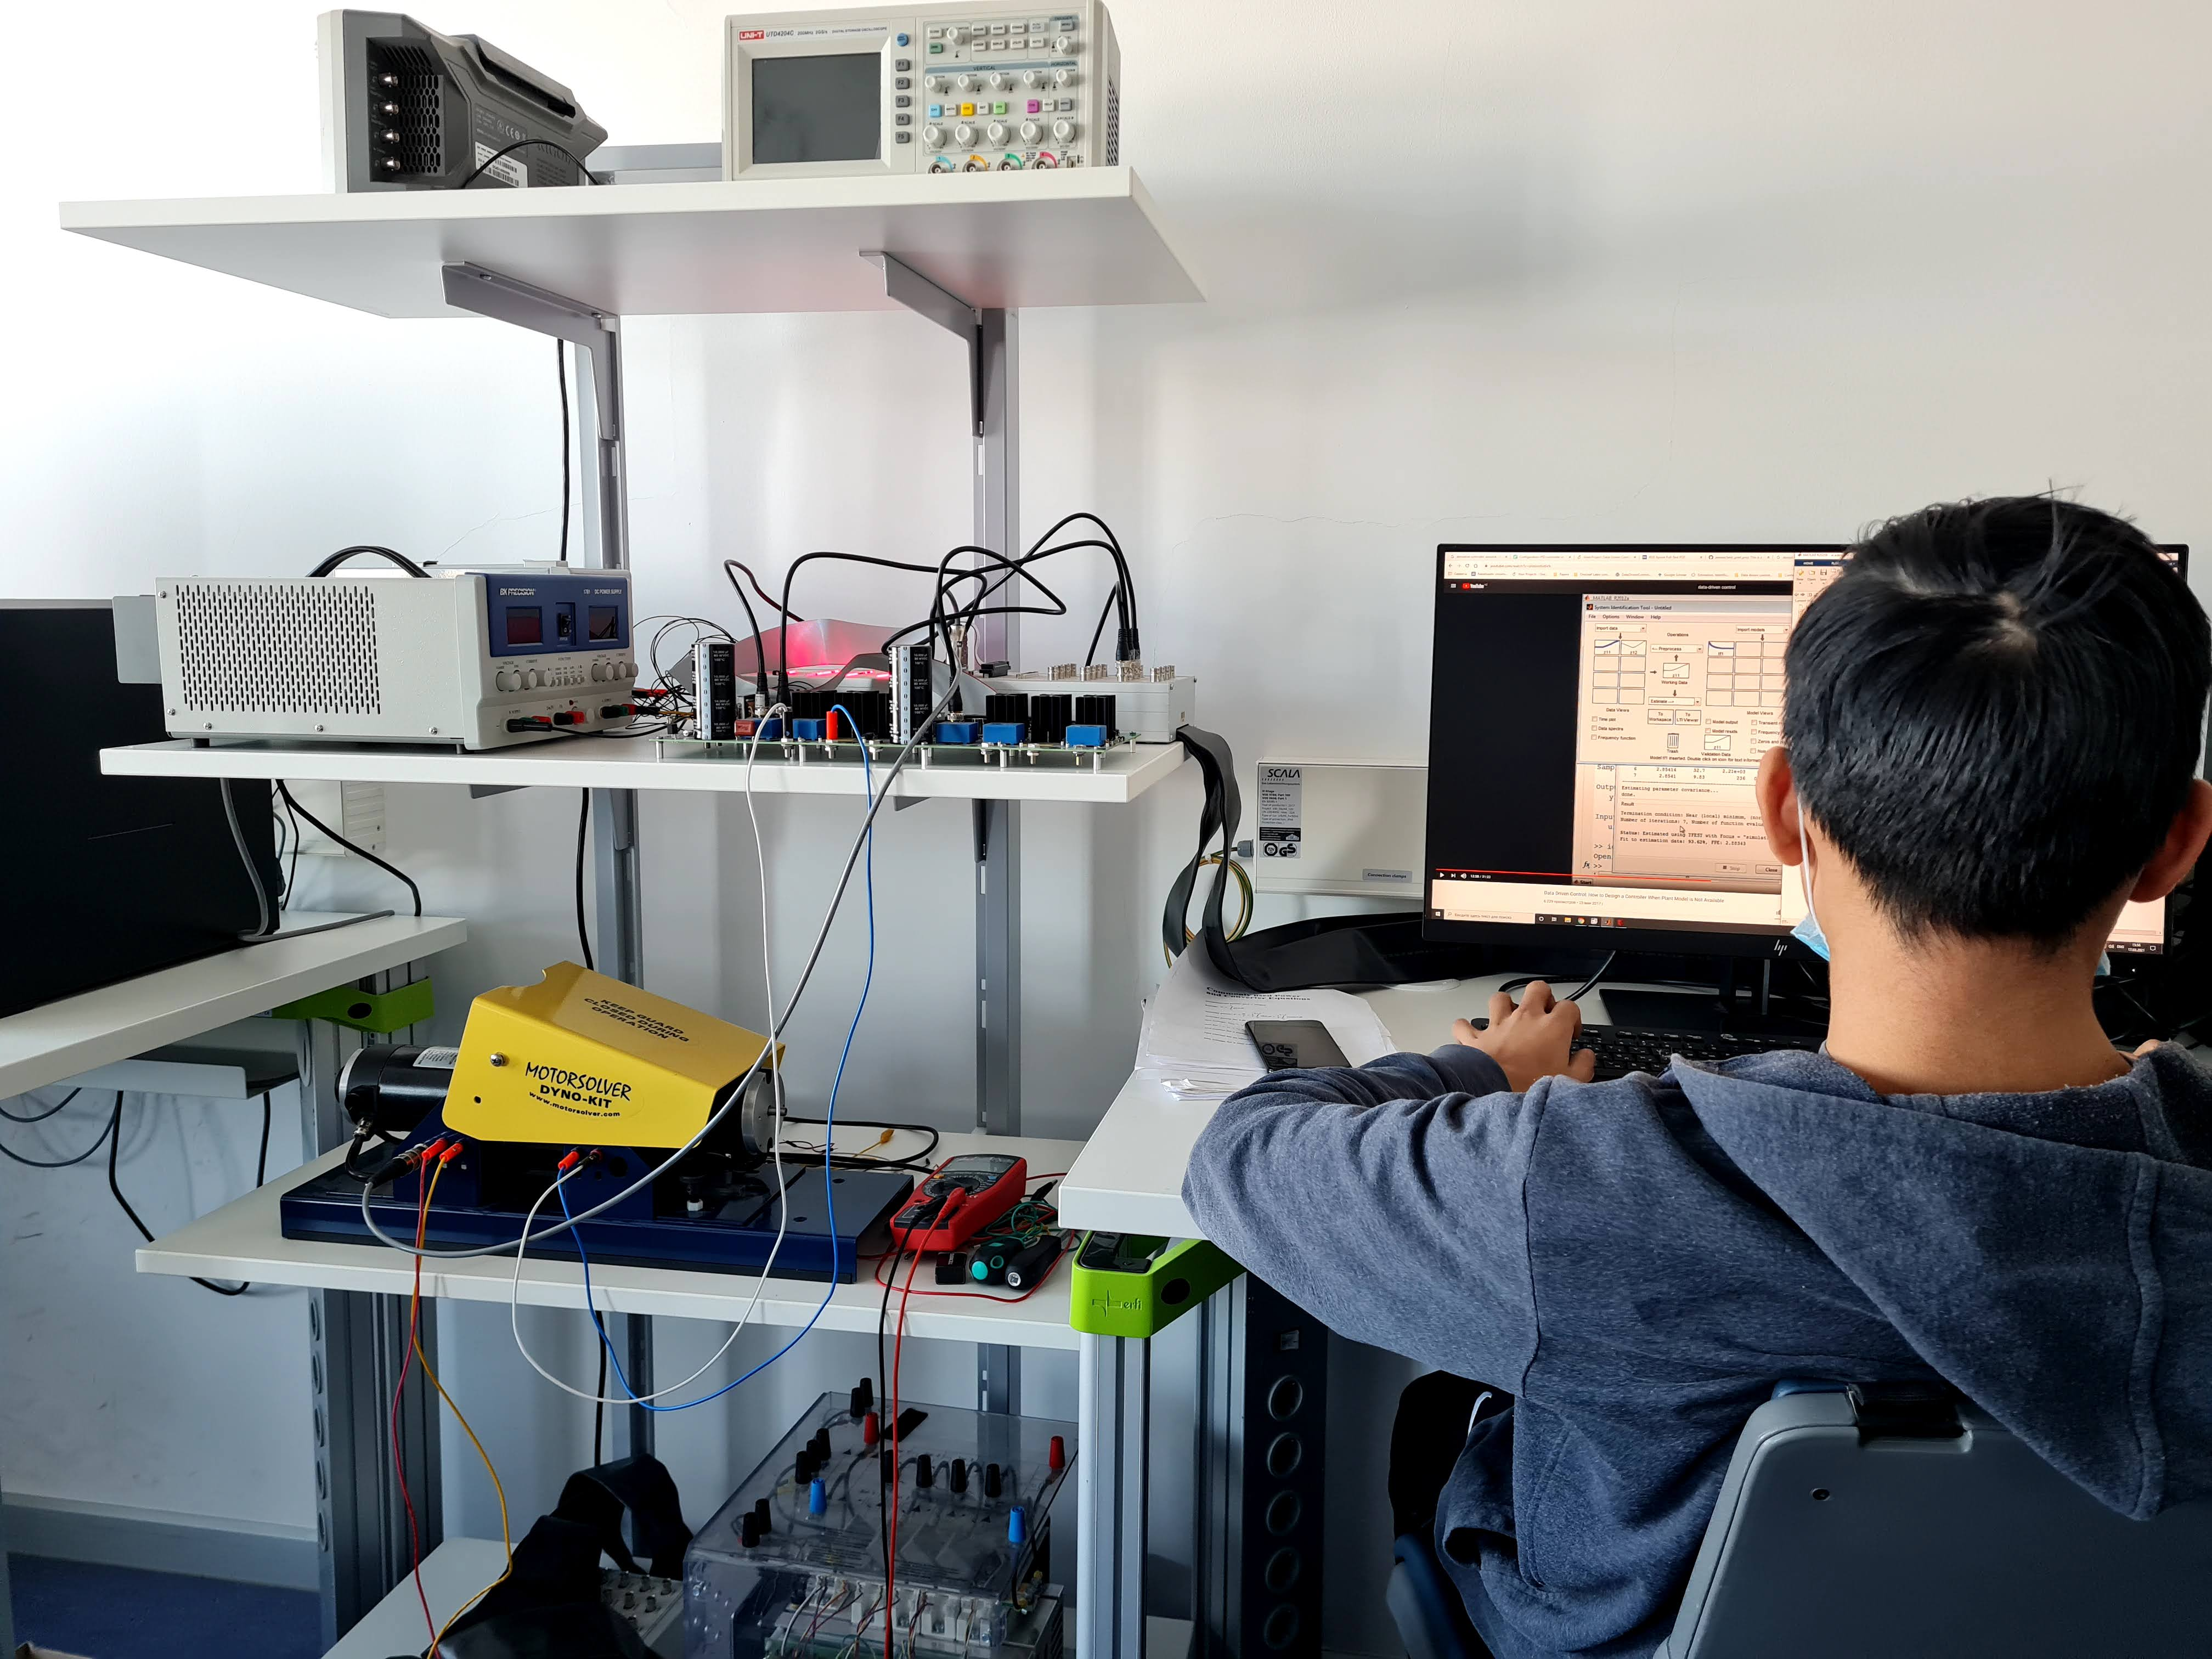
\includegraphics[width=.52\textwidth]{Screenshots for paper/dSpace/dSpace Hardware.jpg}
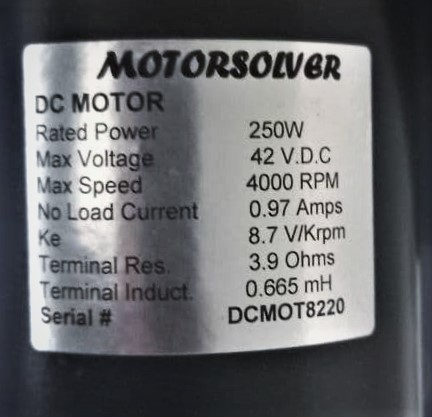
\includegraphics[width=.41\textwidth]{Screenshots for paper/dSpace/motor_specs.jpg}}
\caption{(a) dSpace Hardware setup and (b) the DC motor characteristics}
\label{fig:dSpaceHardware setup}
\end{figure}

The dspace system consists of four parts: the DSpace "ControlDesk" software, DSpace controller board, power electronics board containing the dc-dc converter necessary to drive the motor, and the last the DC motor with the specifications shown in figure \ref{fig:dSpaceHardware setup}. The overall setup is also shown in figure \ref{fig:dSpaceHardware setup}. Overall, the dSpace controller board sends the control signal which represent the amplitude and phase of the PWM signal to the power board and the board in turn generates the according PWM signal which is sent to motor. The motor position is obtained from the Quadrature encoder embedded in the motor. Also the motor current also can be sent as a feedback to further control processing through the ADC. As can be seen from the motor specifications the maximum voltage applied is 42V. The simulink model with which we directly interact shown on the right part of figure \ref{fig:dSpaceEx1} transforms the input signal into the range $\pm$ 21 V. The DSpace controller board operates with sampling time of 0.0001 s.

The model design was implemented in simulink environment within which the Simulink Library provided the I/O interface to the DSpace control board. The built model from simulink is converted and transfered to the DSpace control board. Using the "ControlDesk" software which provides the real-time interface to the input and output signals of the DSpace control board and also to the variables from the simulink model, the input signals of various shapes were applied to motor and were gathered with the corresponding output signal representing the position of motor shaft. The data was used for hardware system identification as was mentioned in the experiment design chapter.

\begin{figure} [h!]
\centerline{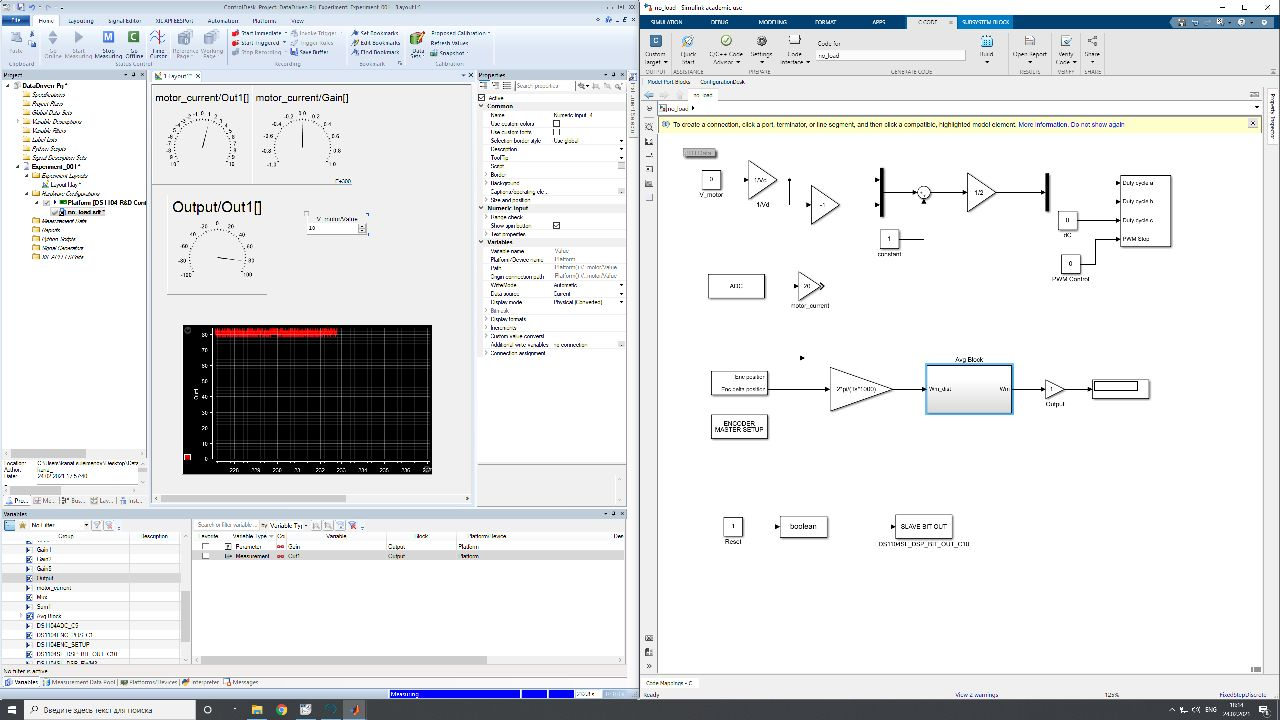
\includegraphics[width=.75\textwidth]{Screenshots for paper/dSpace/photo_2021-03-09 11.37.29.jpeg}}
\caption{dSpace workspace for data gathering}
\label{fig:dSpaceEx1}
\end{figure}


\chapter{Results}
The final obtained results are going to be presented in this chapter. It should be mentioned that currently presented results are intermediate steps results and not the final ones. The final results were not achieved yet due to difficulties with starting the custom PID controller with the dSpace hardware. Overall, it is estimated that currently the project is at 80\% completion state, with the hardware setups constructed and running. The simulation models and the software parts which control the hardware are finished as well. 

\begin{figure} [h!]
\centerline{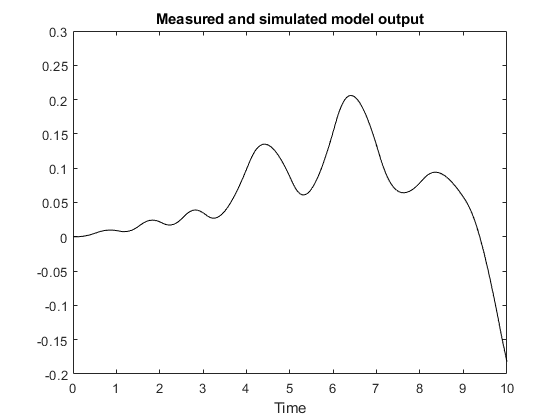
\includegraphics[width=.45\textwidth]{Screenshots for paper/matlab models/simulation_transfer_function_sys_ident.png}
{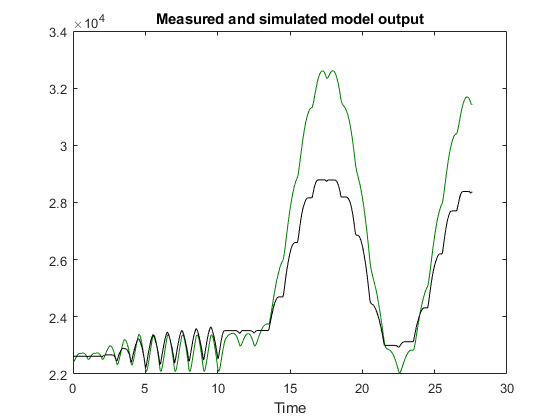
\includegraphics[width=.45\textwidth]{Screenshots for paper/dSpace/hardware_test_sys_ident.png}}
}
\caption{(a) Resultant transfer function match for the MATLAB simulated model and (b) Resultant transfer function match for the dSpace model }
\label{fig:tfresultsim2}
\end{figure}


The above figures represent the results of system identification applied on gathered data from simulation and from hardware experiment. On the left you can see that the generated transfer function of the simscape motor model shows a perfect fit when applied with validation dataset. Whereas the same transfer function model generated from the hardware collected data shows a result of 73\%, although the general dynamics is captured. Arduino setup result were not generated as due to reasons discussed in the Arduino setup chapter. 

\subsection{results from Arduino setup}
The pid controller with the identified model give the controlled signal chasing the reference signal with the settling time being 235 ms.

\begin{figure} [h!]
\centerline{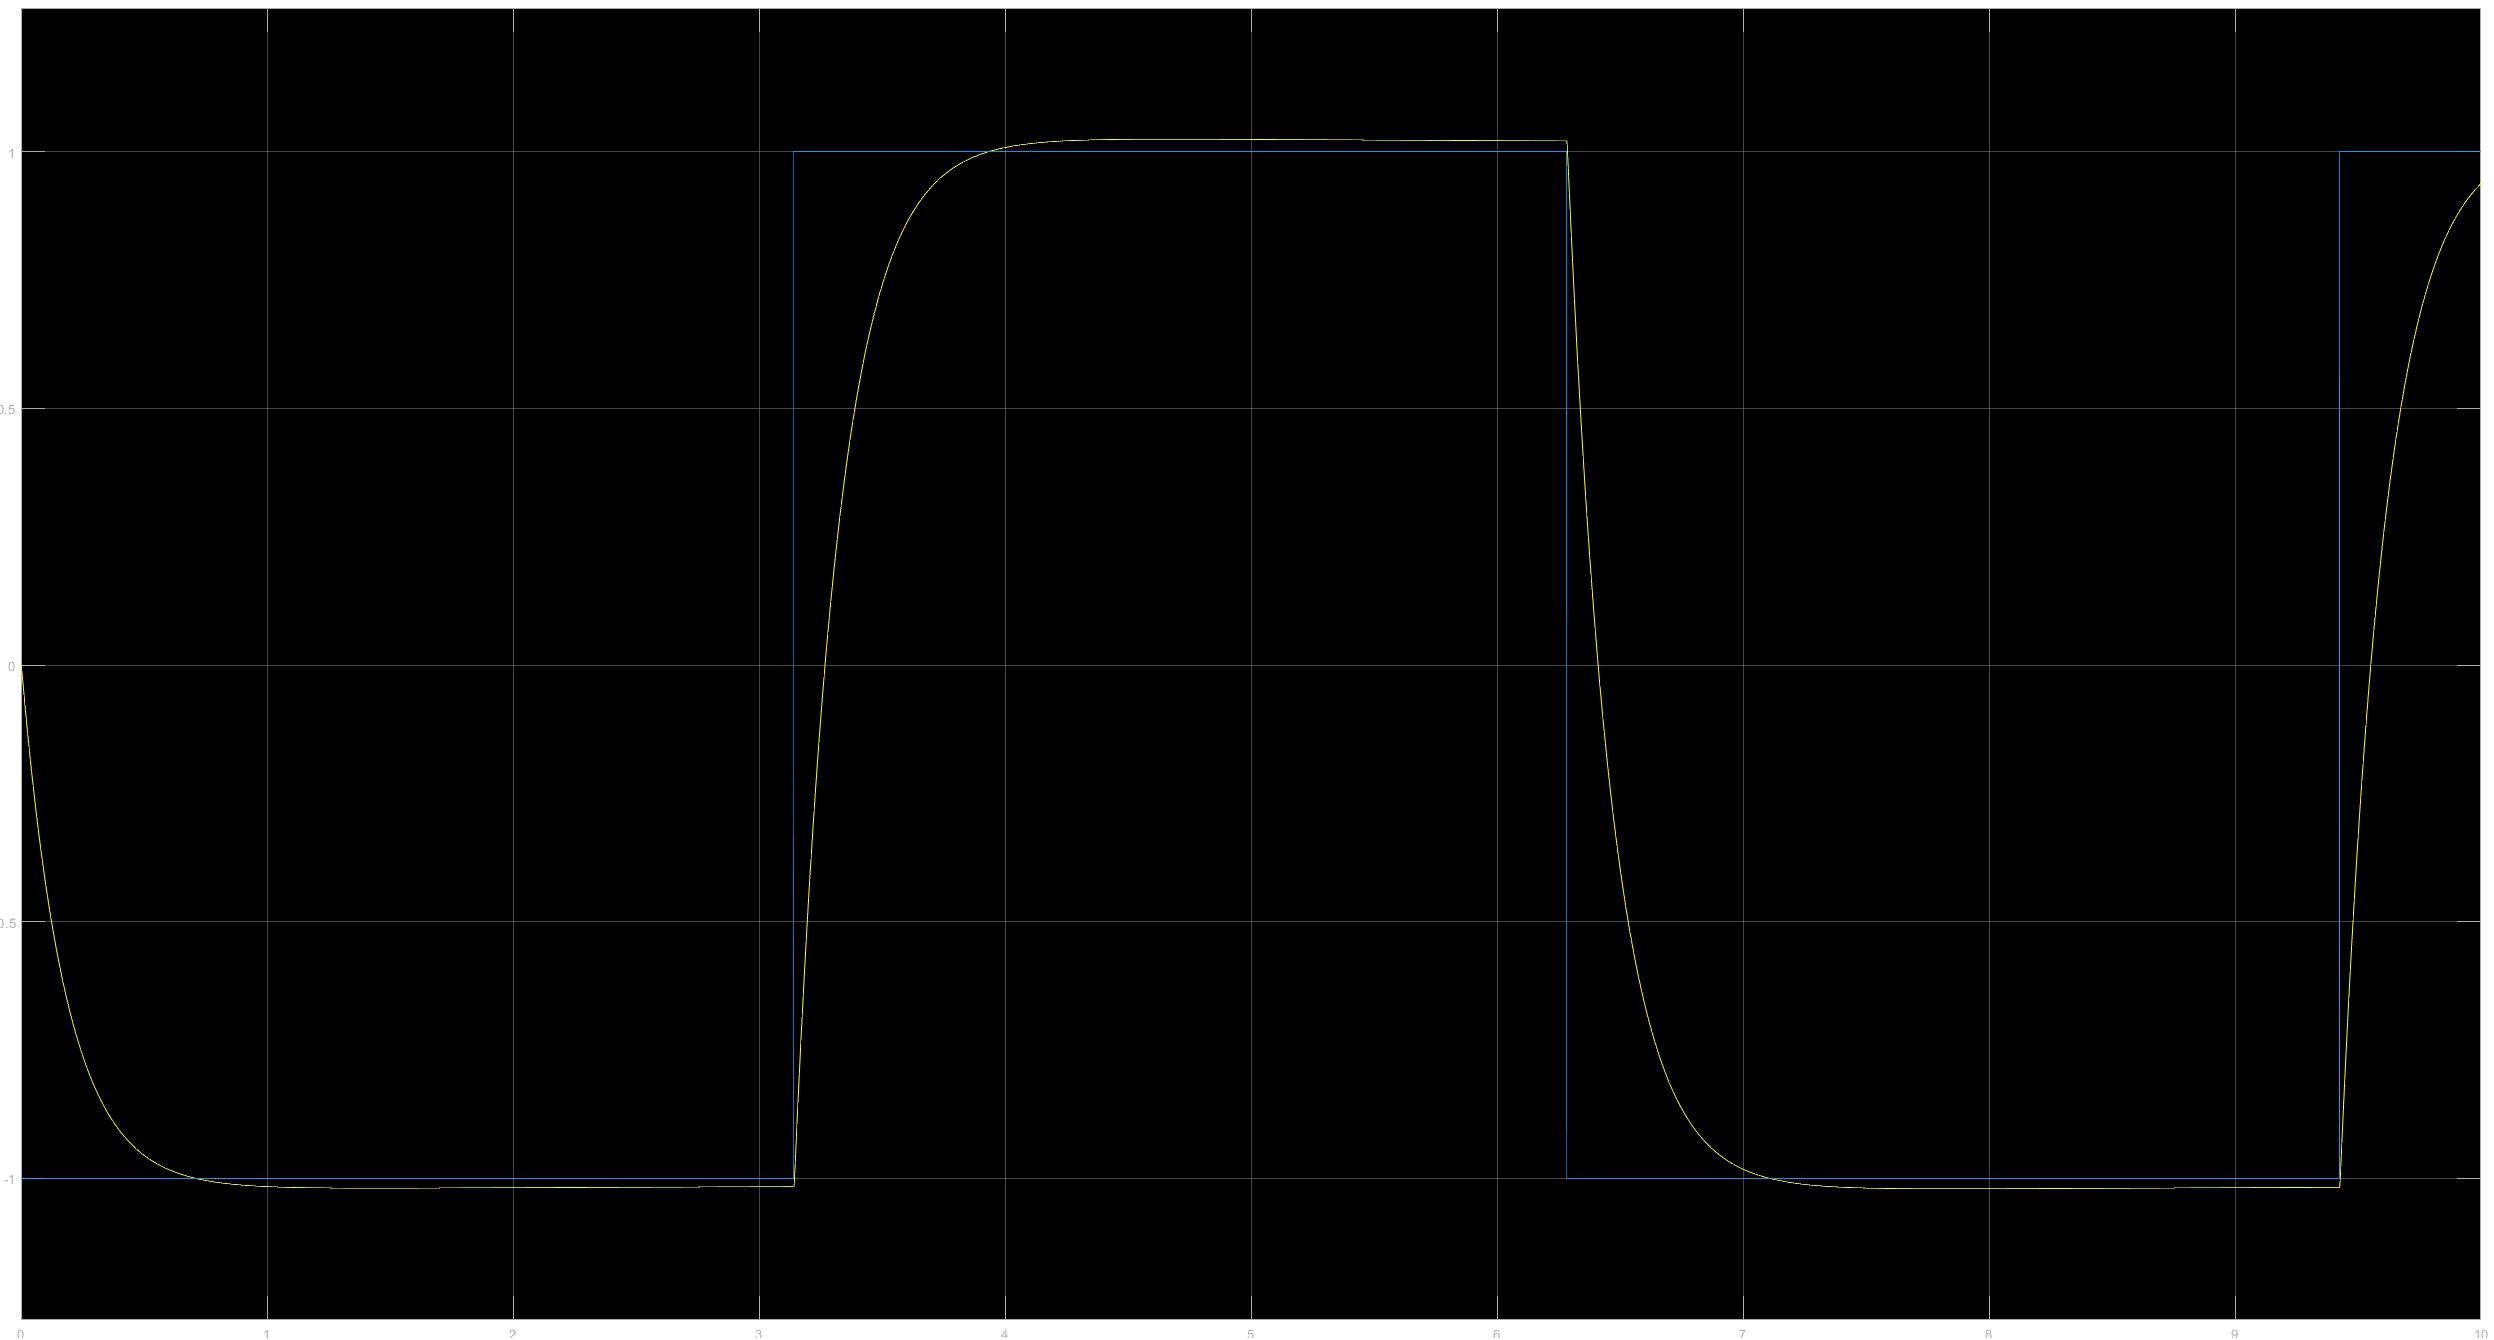
\includegraphics[width=.45\textwidth]{Screenshots for paper/arduino/Final_hardware_testing/square_response.png}
{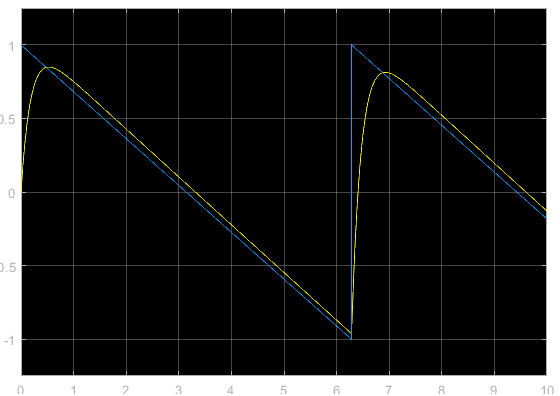
\includegraphics[width=.35\textwidth]{Screenshots for paper/arduino/Final_hardware_testing/untitled.png}}
}
\caption{Control and simulated signal plots for \emph{(a) Results of square} and \textit{(b) Results of sine} waves }
\label{fig:tfresultsim2}
\end{figure}

\chapter{Conclusion and Future work}
We applied the Data-Driven control method to four different setups for this project. A MATLAB simulation, an Arduino, an STM32 and a DC motor driver setup and a dSpace setup were used to generate the DC motor voltage-position relation data. The obtained data was then analyzed in MATLAB system identification toolbox to obtain the tranfer function for the given setup. The ultimate goal of the project - generation of robust controller using data driven approach was achieved with the STM32 setup. While the controller has been generated for the 'solo' Arduino setup as well, the performance was approximately 9 times worse than that of the STM32 setup generated controller. It was not possible to verify the performance of controller for the dSpace setup due to inability of the software provided by manufacturer to include third party controller for the model before running.

A lot of work has been done for the project, however there are still multiple possible extensions for the project that could be taken as a future work. For instance, another method could be used to analyze the obtained data to check if improved inference speed and robustness could be achieved. One of possible variants is the NARX Neural Network, as was suggested in the related work by \cite{naung2018a}.


%%%% ADD YOUR BIBLIOGRAPHY HERE
\newpage
\bibliographystyle{ieeetr}
\bibliography{bibliography} 

\label{endpage}


\end{document}

\end{article}
